\documentclass[journal]{IEEEtran}

%% ─── Packages ────────────────────────────────────────────────────────────────
\usepackage{cite}
\usepackage{amsmath,amssymb,amsfonts}
\usepackage{graphicx}
\usepackage{textcomp}
\usepackage{hyperref}
\usepackage{booktabs}
\usepackage{multirow}
\usepackage{array}
\usepackage{url}
\usepackage{bm}
\usepackage{etoolbox}

% Retained for source compatibility with the tracked draft; final text is black.
\newcommand{\added}[1]{#1}

\hypersetup{
    hidelinks
}

% IEEEtran inserts infinitely stretchable vertical space before no-photo
% biographies. Use compact, fixed separation so short biographies remain
% visually grouped on the final page.
\makeatletter
\patchcmd{\IEEEbiographynophoto}
  {\vskip 4\baselineskip plus 1fil minus 0\baselineskip}
  {\vskip 2\baselineskip}
  {}{}
\makeatother

\def\BibTeX{{\rm B\kern-.05em{\sc i\kern-.025em b}\kern-.08em
    T\kern-.1667em\lower.7ex\hbox{E}\kern-.125emX}}

% NOTE TO AUTHORS: switched from [conference] to [journal] class option, and
% from conference-style \IEEEauthorblockN/\IEEEauthorblockA to the standard
% journal author/affiliation format (with \thanks footnotes), since IEEE
% Transactions on Reliability is a journal, not a conference proceedings venue.

% ─── Document ────────────────────────────────────────────────────────────────
\begin{document}

\title{\added{A Multi-Architecture Neural Operator Digital Twin: A Proof-of-Concept Surrogate Methodology for Cold-Leg LOCA Screening in AP1000 Nuclear Reactors}}

\author{Punyansh~Thakur, Anushka~Paul, Ayush~Kumar~Bhadra, and~Vinay~Kumar
\thanks{P. Thakur and A. Paul are with the Department of Data Science and Artificial Intelligence, IIIT Naya Raipur, Raipur, India (e-mail: punyansh24102@iiitnr.edu.in; anushka24102@iiitnr.edu.in).}
\thanks{A. K. Bhadra is with the Department of Electronics and Communication Engineering, IIIT Naya Raipur, Raipur, India (e-mail: ayush24101@iiitnr.edu.in).}
\thanks{V. Kumar is with the Department of Computer Science and Engineering, IIIT Naya Raipur, Raipur, India (e-mail: vinay@iiitnr.edu.in). Corresponding author: V. Kumar.}}

\markboth{IEEE Transactions on Reliability,~Vol.~XX, No.~XX, 2026}%
{\added{Thakur \MakeLowercase{\textit{et al.}}: A Multi-Architecture Neural Operator Digital Twin for Cold-Leg LOCA Screening in AP1000 Nuclear Reactors}}

\maketitle

%─── Abstract ─────────────────────────────────────────────────────────────────
\begin{abstract}

\added{High-fidelity computational-fluid-dynamics (CFD) analysis is generally too costly for repeated online accident-screening studies. This paper presents an artifact-traceable, proof-of-concept AP1000 digital-twin methodology that couples spatial surrogate modeling to a plant-indicator classifier. Three neural operators map inlet velocity, a prescribed break-severity proxy, and coolant temperature to pressure, velocity magnitude, turbulent kinetic energy, and temperature on a shared 25,000-point mesh: DeepONetFourier (1,451,012 parameters), a Transolver-inspired token operator (3,244,872), and a grade-structured Clifford-algebra operator (37,380). The benchmark comprises 2,000 physics-inspired analytic synthetic cases, of which 300 are held out for testing. DeepONetFourier achieved pooled $R^2$ values of 0.9961, 0.9958, 0.9951, and 0.9962 for the four normalized fields, respectively; a separate seed-42 Transolver-inspired run achieved 0.9918, 0.9932, 0.9806, and 0.9951. The three archived checkpoints also provide matched-scale qualitative reconstructions, and a dataset-matched unmodified DeepONet baseline is reported. Because the objectives are not identical, these results establish architecture-specific feasibility rather than a controlled accuracy ranking. Separately, a gradient-boosting classifier trained on open PCTRAN-simulated NPPAD records with synthetic transition augmentation achieved ROC-AUC 0.990554 and recall 0.989063 on one fixed row-level split. A translation-path diagnostic verifies executable coupling, although its label-conditioned break input precludes interpretation as independent accident diagnosis. Together, the results demonstrate a reproducible multi-architecture workflow under the analytic benchmark. Full-fidelity CFD or experimental validation, label-independent group-separated detection tests, and reliability-oriented operating-point analysis remain necessary before safety-relevant assessment.}
\end{abstract}

\begin{IEEEkeywords}
AP1000, Clifford algebra, DeepONet, digital twin, Fourier features, LOCA screening, neural operators, nuclear safety, surrogate modeling, Transolver
\end{IEEEkeywords}A

%═══════════════════════════════════════════════════════════════════════════════
\section{Introduction}
%═══════════════════════════════════════════════════════════════════════════════

\added{The AP1000 is a Generation~III+ pressurized-water reactor designed by Westinghouse with passive safety features. A cold-leg loss-of-coolant accident (LOCA) is a postulated rupture in the primary coolant return piping whose safety analysis requires system-level thermal-hydraulic modeling, uncertainty treatment, and comparison with applicable evidence \cite{wecdcd,nrc_loca}. This study investigates data-driven reconstruction and screening as a research supplement; it does not replace engineered protection, qualified analysis codes, or operator authority.}

\added{High-fidelity CFD can predict spatial thermohydraulic states, but its computational cost limits repeated online evaluation.} Neural operators---machine-learning models that learn mappings between function spaces---have emerged as PDE surrogates. Lu et al.~\cite{lu2021deeponet} introduced Deep Operator Networks (DeepONet), decomposing the solution operator $\mathcal{G}: \mathcal{U} \to \mathcal{V}$ via a branch--trunk factorization. \added{The coordinate MLP in the present baseline is susceptible to spectral bias \cite{rahaman2019spectral} and uses fixed ReLU activations. The studied extension adds Fourier coordinates, adaptive activations, and serialized-node smoothness proxies; Section~\ref{sec:deeponet_fourier} defines their scope explicitly.}

Subsequent work has explored alternative neural operator paradigms: Transolver~\cite{wu2024transolver} applies transformer attention to mesh-compressed tokens for general-geometry PDE solving, and Clifford Neural Operators~\cite{brandstetter2023clifford} use geometric-algebra representations to encode grade structure. \added{Recent nuclear applications include DeepONet-based hot-leg virtual sensing and DeepONet/FNO surrogates for a helical-coil steam generator \cite{hossain2025virtual,lee2026hcsg}. A documented public-source search found no prior study that jointly evaluates Transolver- and Clifford-style operators in a cold-leg LOCA field-surrogate-to-classifier workflow. The novelty claimed here is this specific, multi-architecture integration and evaluation scope.}

\added{The Fourier Neural Operator (FNO) \cite{li2021fno} is a natural comparison candidate. The present study instead focuses on branch--trunk, token-attention, and Clifford-algebra parameterizations under one fixed point-cloud representation. An FNO benchmark with a documented gridding/interpolation protocol is reserved for a controlled follow-up.}

The main contributions of this paper are summarized as follows:
\begin{enumerate}
    \item \added{We design and implement three neural-operator architectures---an upgraded DeepONetFourier, a Transolver-inspired token operator, and a Clifford-algebra operator---within a unified proof-of-concept pipeline for LOCA screening.}
    \item We introduce four changes to baseline DeepONet---random Fourier feature encoding ($\sigma = 10.0$, $m = 256$), per-neuron adaptive GELU activations, an index-gradient matching term ($\beta = 0.1$), and a velocity-variation term ($\lambda = 0.01$)--- \added{reducing the measured parameter count from 3,162,116 to 1,451,012 (54.1\%)} under the synthetic benchmark. \added{The latter two terms are serialized-node regularizers rather than geometry-aware physics derivatives.}
    \item \added{We evaluate the Transolver-inspired operator (mesh-token attention with $M = 64$ tokens, 3,244,872 parameters) and the grade-structured Clifford-algebra operator (37,380 parameters) as complementary field surrogates.}
    \item \added{We provide an artifact-backed comparison along the dimensions supported uniformly across the three implementations: architecture, parameter count, objective, output interface, and matched-scale qualitative reconstruction. Quantitative accuracy is reported where a complete evaluation artifact is available.}
    \item \added{We couple the surrogate models to a LOCA indicator-translation demonstration. The archived single-split classifier reaches ROC-AUC 0.990554 on PCTRAN-simulated NPPAD data with synthetic transition augmentation, and a five-seed diagnostic verifies the executable translation path.}
\end{enumerate}

\added{These contributions are evaluated as a reproducible feasibility study. Claims of physical conservation, architecture ranking, and independent accident diagnosis are deliberately excluded because the present artifacts do not support them.}

The remainder of this paper is organized as follows. Section~\ref{sec:related} reviews related work on neural operators and machine learning for nuclear power plant safety. Section~\ref{sec:problem} formulates the surrogate-modeling problem and its input-output specification. Section~\ref{sec:system} describes the end-to-end system architecture and the five-stage digital twin pipeline. Section~\ref{sec:architectures} details the three neural operator architectures and their respective improvements over baseline DeepONet. Section~\ref{sec:pipeline} presents the downstream LOCA indicator detection pipeline, including the NPPAD feature mapping and severity model. Section~\ref{sec:impl} describes implementation details, software, hardware, and the training protocol. Section~\ref{sec:results} reports experimental results under the synthetic benchmark. Section~\ref{sec:discussion} discusses the methodological contributions, architectural trade-offs, and the limitations that define the path to full-fidelity validation. Section~\ref{sec:conclusion} concludes the paper.

%═══════════════════════════════════════════════════════════════════════════════
\section{Related Work}
\label{sec:related}
%═══════════════════════════════════════════════════════════════════════════════

\subsection{Neural Operators and DeepONet}
\added{Neural operators learn mappings between function spaces \cite{lu2022comprehensive}. Two widely used families are the Fourier Neural Operator (FNO) \cite{li2021fno}, whose standard FFT realization uses a regular grid, and DeepONet \cite{lu2021deeponet,chen1995}, which factorizes the learned mapping into branch and trunk networks and can query arbitrary coordinates. Coordinate MLPs can preferentially fit low-frequency components \cite{rahaman2019spectral}; Fourier feature encoding \cite{tancik2020ffn} and derivative-aware training \cite{son2021sobolev} are two relevant remedies.}

\subsection{Transformer and Geometric Neural Operators}
Transolver \cite{wu2024transolver} compresses $N$-node meshes to $M \ll N$ learned tokens via soft-assignment attention, achieving $\mathcal{O}(M^2)$ token-attention complexity; GNOT \cite{hao2023gnot} applies a related transformer-based approach to operator learning. Clifford Neural Operators \cite{brandstetter2023clifford} take a different route by embedding physical fields in Clifford algebra.  \added{Equivariance depends on maintaining grade-respecting operations through the output map; the implementation studied here uses a dense grade-mixing readout, so it is described as grade-structured rather than exactly equivariant. The domain-novelty statement is limited to the targeted-search scope stated in Section~I.}

\subsection{Machine Learning for Nuclear Power Plant Safety}
\added{Machine-learning research for nuclear reactors spans transient classification, fault diagnosis, sensor monitoring, and thermal-hydraulic surrogates, while important barriers include limited representative data, distribution shift, robustness, and interpretability \cite{huang2023review}. Digital-twin concepts emphasize a maintained connection between physical and digital assets \cite{grieves2014}; recent nuclear virtual-sensing work illustrates this direction with neural operators \cite{hossain2025virtual}. The present work connects analytic spatial-field surrogates to an ML classifier in a unified proof-of-concept workflow and, within the targeted-search scope above, compares multiple operator paradigms for cold-leg LOCA screening.}

\subsection{Reliability-Engineering Perspective on AI-Based Detection}
\label{sec:related_reliability}


\added{Reliability-oriented fault detection is evaluated through an operating characteristic, not a single accuracy number. Probability of detection and false-alarm rate must be reported as functions of the threshold and operating regime because their consequences are asymmetric \cite{isermann2005}. The single threshold used here is therefore descriptive; it is not a justified alarm setting.}

\added{For safety-relevant software, IEEE Std~1012 defines lifecycle V\&V processes, while recent nuclear guidance emphasizes trustworthy design, data governance, testing, monitoring, human oversight, and defense in depth for AI applications \cite{ieee1012,nrc7294,trilateral2024}. These sources motivate a staged safety case comprising requirements traceability, independent test evidence, uncertainty and distribution-shift analysis, configuration control, and documented human authority. The present prototype supplies none of the evidence needed for certification and is not proposed for plant protection or autonomous actuation.}

\added{Validation maturity must also be separated by model class. Nuclear thermal-hydraulic system codes such as TRACE and RELAP5 have long-established assessment practices against qualified experimental databases and plant transients; best-estimate-code qualification explicitly addresses code, user, nodalization, and uncertainty effects \cite{petruzzi2008,nrc_codes}. In contrast, this work evaluates spatial surrogates only against an analytic mock generator. Its contribution is architectural and workflow-level feasibility, not parity with a qualified system-code analysis.}

%═══════════════════════════════════════════════════════════════════════════════
\section{Problem Formulation}
\label{sec:problem}
%═══════════════════════════════════════════════════════════════════════════════

\added{Let $\Omega \subset \mathbb{R}^3$ denote the evaluated straight cylindrical cold-leg proxy segment, with diameter $D = 0.7$\,m and length $10D$. The analytic benchmark does not include the elbow geometry present in the planned Fluent model.} Define the parameter vector $\bm{u} = [v, b, T]^\top \in \mathbb{R}^3$, where $v \in [4.0, 6.0]$\,m/s is the inlet velocity, $b \in [0, 10]$\% is the \added{prescribed break-severity proxy}, and $T \in [290, 320]^\circ$C is the coolant temperature. \added{In the evaluated generator, $b$ modulates closed-form fields; no physical opening or break-area mesh is resolved.}

\added{The evaluated goal is to learn the parametric mapping defined by the analytic generator; future CFD validation would replace these targets with independently verified solver fields:}
\begin{equation}
\mathcal{G}_\theta(\bm{u})(\bm{y}) = \hat{\bm{s}}(\bm{y}) = [\hat{p},\; |\hat{\bm{v}}|,\; \hat{k},\; \hat{T}]^\top \in \mathbb{R}^4
\label{eq:operator}
\end{equation}
for every spatial location $\bm{y} \in \Omega$, evaluated simultaneously across $N = 25{,}000$ mesh nodes: output $\hat{\bm{S}} \in \mathbb{R}^{B \times 4 \times N}$.  \added{The stored dataset and model output contain these four scalar fields only; no $(v_x,v_y,v_z)$ tensor is produced. Consequently, the implemented velocity regularizer cannot represent $\nabla\!\cdot\!\bm v$ or establish mass conservation. Section~\ref{sec:deeponet_fourier} therefore defines it as a serialized-node velocity-variation proxy and identifies geometry-aware vector conservation as future work.}

\subsection{Analytic Synthetic-Benchmark Setup}

\added{The evaluated generator assumes constant coolant density of 720\,kg/m$^3$ and a 15.5\,MPa pressure scale. It does not solve the RANS equations. Instead, closed-form axial, radial, and break-localized expressions generate pressure, velocity magnitude, turbulent kinetic energy, and temperature on the straight cylindrical proxy mesh, with small stochastic perturbations. The dataset comprises 2,000 parameter combinations: 20 velocity $\times$ 10 break-size $\times$ 10 temperature levels, split deterministically with seed~42 into training (1,400), validation (300), and test (300) samples.}

Accordingly, the present benchmark should be interpreted as a parametric field-regression proxy with operator-learning structure rather than a fully validated PDE-solution benchmark.

%═══════════════════════════════════════════════════════════════════════════════
\section{System Architecture and Pipeline}
\label{sec:system}
%═══════════════════════════════════════════════════════════════════════════════

The digital twin operates as a five-stage cascade pipeline (Fig.~\ref{fig:pipeline}), with each stage transforming data from one physical or learned representation into the next, culminating in a LOCA classifier score for screening research. A master controller orchestrates the cascade and supports runtime selection of any neural operator architecture through a unified configuration interface.

\begin{figure*}[htbp]
\centering
\fbox{\parbox{0.96\textwidth}{\centering\small
\textbf{Stage~1: Data Generation} \\[2pt]
\added{Evaluated analytic generator $\;\longrightarrow\;$ 2{,}000 cases $\times$ 25{,}000 nodes $\times$ (3 coordinates + 4 retained fields)} \\[6pt]
$\downarrow$ \\[4pt]
\textbf{Stage~2: Preprocessing \& Normalization} \\[2pt]
CSV $\to$ HDF5: Branch $\bm{U}\!\in\!\mathbb{R}^{2000\times 3}$, Trunk $\bm{Y}\!\in\!\mathbb{R}^{25000\times 3}$, Targets $\bm{S}\!\in\!\mathbb{R}^{2000\times 4\times 25000}$ \quad$\mid$\quad MinMaxScaler per field \\[6pt]
$\downarrow$ \\[4pt]
\textbf{Stage~3: Neural Operator Training} \\[2pt]
\added{DeepONetFourier $\xrightarrow{\text{MSE + serialized-node proxies}}$ \texttt{deeponet\_fourier\_best.pth}; token/Clifford operators $\xrightarrow{\text{MSE}}$ architecture-specific checkpoints.} \\[6pt]
$\downarrow$ \\[4pt]
\textbf{Stage~4: LOCA Indicator Classifier Training} \\[2pt]
 \added{Open PCTRAN-simulated NPPAD data (302 Normal + 45{,}176 LOCA rows) + 3{,}800 synthetic transition samples} $\to$ GBC/MLP $\to$ \texttt{loca\_detector.pkl} \\[6pt]
$\downarrow$ \\[4pt]
\textbf{Stage~5: Inference Pipeline (Screening Mode)} \\[2pt]
$\bm{u}\!\to$ Normalize $\to$ Neural Operator $\to$ Denormalize $\to$ Feature Extraction $\to$ NPPAD Mapping $\to$ LOCA Classifier $\to$ $S_{\text{LOCA}}$ \\[2pt]
\added{\textbf{Single-case timing path available; reproducible matched-hardware benchmark deferred.}}
}}
\caption{End-to-end digital-twin proof-of-concept pipeline. Stages 1--4 run offline and Stage~5 executes the screening demonstration. \added{The evaluated field data are synthetic, NPPAD records are PCTRAN-simulated, and this workflow is neither a plant protection system nor an operationally validated digital twin.}}
\label{fig:pipeline}
\end{figure*}

\subsection{\added{Stage~1: Parametric Field-Data Generation}}

The training data originate from a parametric sweep of the three-dimensional input space $(v, b, T)$. Two data-generation pathways are supported:

\textbf{\added{Pathway A --- ANSYS Fluent Automation (Unevaluated Prototype):}}
\added{The repository includes a journal-generation prototype that can configure a steady pressure-based solver, RNG $k$--$\varepsilon$ closure, inlet/outlet conditions, a pre-existing break boundary zone, 1,000 solver iterations, and CSV field export. This pathway did not produce the dataset or results reported in this paper. Before it can serve as a validation path, the geometry and break-area parameterization, mesh independence, solver convergence, and export consistency must be verified in Fluent.}

\textbf{\added{Pathway B --- Analytic Synthetic Generator (Evaluated):}}
A synthetic data generator produces fields on a shared 25,000-node mesh (cylindrical pipe, diameter $D = 0.7$\,m, length $10D$) incorporating:
\begin{itemize}
    \item \added{\textbf{Pressure}: Linear axial term ($\Delta p = 50{,}000 \cdot v/5$ Pa) + localized Gaussian break-proxy drop ($200{,}000 \cdot b_\text{norm}$ Pa, $\sigma = 0.8$\,m) + prescribed radial shape term ($5{,}000(1-r^2)$ Pa)}
    \item \textbf{Velocity}: Parabolic profile $v(r) = v_\text{in}(1 - r^{\alpha})$, with $\alpha = 2 - 0.8 b_\text{norm} e^{-\frac{(x - x_\text{break})^2}{2\sigma^2}}$ (flattens near break) and 30\% reduction at full break
    \item \textbf{Turbulence}: Base $k = 0.01 v^2$, wall-layer increase (factor $1 + 1.5r$), break-induced spike ($5 b_\text{norm}$, localized at break)
    \item \textbf{Temperature}: Kelvin base + radial gradient ($3(1-r^2)$\,K) + downstream break hot-spot ($15 b_\text{norm}$\,K) + axial cooling (2\,K over pipe length)
\end{itemize}
where $b_\text{norm} = b/10 \in [0,1]$ and $r = \sqrt{y^2 + z^2}/(D/2)$ is the normalized radial position. \added{The fields include small Gaussian or uniform stochastic perturbations specified by the generator; these perturbations are heuristic and are not a turbulence model.}

The 2,000 parameter combinations form a $20 \times 10 \times 10$ structured grid: 20 velocity levels in $[4.0, 6.0]$\,m/s, 10 break sizes in $[0, 10]$\%, and 10 temperatures in $[290, 320]^\circ$C.

\subsection{Stage~2: Preprocessing and Normalization}

The \texttt{DeepONetDataPreprocessor} module converts raw CSV files into a training-ready HDF5 dataset:

\begin{enumerate}
    \item \textbf{Loading}: Each CSV is parsed into a DataFrame, source headers are mapped to consistent internal field names, and mesh consistency is checked across all simulations ($N=25{,}000$ nodes).
    
    \item \textbf{Tensor construction}:
    \begin{align}
    \bm{U} &\in \mathbb{R}^{2000 \times 3} && \text{(branch inputs: $v,b,T$)}, \\
    \bm{Y} &\in \mathbb{R}^{N \times 3} && \text{(trunk inputs: $x,y,z$)}, \\
    \bm{S} &\in \mathbb{R}^{2000 \times 4 \times N} && \text{(target fields)}.
    \end{align}
    
    \item \textbf{Normalization}: Per-field MinMaxScaler to $[0,1]$. Branch inputs are scaled jointly; trunk coordinates are scaled jointly; each target field (pressure, velocity, turbulence, temperature) receives its own independent scaler. All fitted scalers are serialized (pickled) for use during inference denormalization.
    
    \item \added{\textbf{Splitting}: Deterministic random 70/15/15\% split into training (1,400), validation (300), and test (300) samples using seed~42. No label stratification is applied. The trunk coordinates $\bm{Y}$ are shared across all splits (same mesh for all simulations).}
    
    \item \textbf{Storage}: The splits are saved to a single HDF5 file (\texttt{deeponet\_dataset.h5}) with groups \texttt{train/}, \texttt{val/}, \texttt{test/}, each containing datasets \texttt{branch}, \texttt{trunk}, \texttt{targets}.
\end{enumerate}

\subsection{Stage~3: Neural Operator Training}

The training stage supports three interchangeable neural operator architectures (detailed in Section~\ref{sec:architectures}). The architecture is selected at runtime via a \texttt{model\_config.yaml} configuration file, with all operators sharing the same data loader and evaluation metrics.

\textbf{Data loading}: A PyTorch \texttt{Dataset} reads HDF5 lazily. Each sample is a tuple (branch~$\bm{u}_i \in \mathbb{R}^3$, trunk~$\bm{Y} \in \mathbb{R}^{N \times 3}$, targets~$\bm{s}_i \in \mathbb{R}^{4 \times N}$). \added{The standard DeepONetFourier and Tier-2 drivers, as well as the reported Transolver-inspired run, use $B=4$.}

\textbf{Training loop}: For each batch:
\begin{enumerate}
    \item Forward pass: $\hat{\bm{S}} = \mathcal{G}_\theta(\bm{U}_\text{batch}, \bm{Y})$ $\in \mathbb{R}^{B \times 4 \times N}$
    \item Loss computation:  \added{In the executed DeepONetFourier path, the base MSE is added to a ``Sobolev'' module that itself contains an MSE term plus a central-difference term along stored node index. A second module applies the same index difference to velocity magnitude. Thus, with $D_{\mathrm{idx}}$ denoting that serialized-node difference, the effective objective is}
    {
    \begin{equation}
    \begin{aligned}
    \mathcal{L}_{\mathrm{DF}} ={}& 2\,\mathcal{L}_{\mathrm{MSE}}
      + \beta \left\|D_{\mathrm{idx}}\hat{\bm S}-D_{\mathrm{idx}}\bm S\right\|_F^2 \\
      &+ \lambda \left\|D_{\mathrm{idx}}|\hat{\bm v}|\right\|_F^2,
    \end{aligned}
    \label{eq:total_loss}
    \end{equation}}
    \added{where $\beta=0.1$ and $\lambda=0.01$. Because the mesh rows are not ordered as a physical one-dimensional stencil, the latter terms are smoothness proxies, not $\nabla\bm S$ and $\nabla\!\cdot\!\bm v$. The Transolver-inspired and Clifford-algebra operators use MSE only.}
    \item Backward pass with Automatic Mixed Precision (AMP) arithmetic (FP16 forward, FP32 gradients)
    \item Adam optimizer step with gradient clipping ($\|\nabla\theta\|_\text{max} = 1.0$)
\end{enumerate}

\textbf{Scheduling}: DeepONetFourier uses ReduceLROnPlateau (patience~20, factor~0.5) and effective early stopping with patience~50. The Tier-2 driver uses CosineAnnealingLR and configures patience~50; however, its original Boolean return-value check was ineffective, so early stopping was inactive in the reported Transolver-inspired run.

\textbf{Evaluation metrics}: Per-field $R^2$, relative $L_2$ error, and MAE are computed on validation/test data; the exact pooled test definitions used in Table~\ref{tab:field_metrics} are stated there.  \added{The evaluated checkpoints are architecture-specific: \texttt{deeponet\_fourier\_best.pth}, \texttt{transolver\_best.pth}, and \texttt{clifford\_best.pth}.}

\subsection{Stage~4: LOCA Indicator Classifier Training}

The \texttt{LOCADetector} module trains a supervised binary classifier completely independently from the neural operator.

\textbf{Data source}:  \added{The open Nuclear Power Plant Accident Database (NPPAD), generated with the PCTRAN simulator rather than measured at an operating plant} \cite{qi2022nppad}, is loaded from the \texttt{data/nppad/operation\_csv\_data/} directory:
\begin{itemize}
    \item \texttt{Normal/} --- 1 CSV, 302 timestep rows (steady-state operation)
    \item \texttt{LOCA/} --- 100 CSVs, $\sim$45,176 timestep rows (accident transients)
\end{itemize}

\textbf{Feature extraction}: Seven NPPAD signals are selected from each row: primary pressure~$P$, average temperature~$T_\text{avg}$, RCS flow~$W_\text{RCA}$, SG-A pressure~$P_\text{SGA}$, subcooling margin~$\Delta T_\text{sub}$, Departure from Nucleate Boiling Ratio (DNBR), and hot-cold leg temperature differential $\Delta T_\text{HL-CL} = T_\text{HA} - T_\text{CA}$.

\textbf{Transitional data augmentation}:  \added{To avoid an exclusively endpoint-like training distribution,} 19 severity levels $s \in \{0.05, 0.10, \ldots, 0.95\}$ are generated with 200 samples each. At each level, feature values are interpolated between Normal and LOCA distributions, with labels drawn as Bernoulli($s$). This adds 3,800 synthetic samples, giving 49,278 rows before the split. \added{This construction does not establish probability calibration.}

\textbf{Classifier}: A Gradient Boosting Classifier (200 trees, depth~4, learning rate~0.05, min.\ 20 samples/leaf) trained on StandardScaler-normalized features. \added{An 80/20 stratified row-level split with seed~42 is used for training and evaluation. It is not grouped by source transient; consequently, the reported score is a within-dataset classifier result rather than an unseen-transient validation.}

\textbf{Artifacts}: The trained model, scaler, and metrics are serialized to \texttt{loca\_detector.pkl}.

\subsection{Stage~5: Inference Pipeline (Screening Mode)}
\label{sec:inference_pipeline}

The \texttt{DigitalTwinInference} class orchestrates the forward pass through the complete digital twin at runtime. The five steps execute sequentially within each inference call:

\textbf{Step~1 --- Input normalization}: Physical parameters $(v, b, T)$ are transformed using the branch MinMaxScaler from Stage~2:
\begin{equation}
\bm{u}_\text{norm} = \frac{\bm{u} - \bm{u}_\text{min}}{\bm{u}_\text{max} - \bm{u}_\text{min}} \in [0,1]^3
\end{equation}

\textbf{Step~2 --- Neural operator forward pass}: The normalized branch input and pre-stored normalized trunk coordinates are fed to the loaded neural operator:
\begin{equation}
\hat{\bm{S}}_\text{norm} = \mathcal{G}_\theta(\bm{u}_\text{norm}, \bm{Y}_\text{norm}) \in \mathbb{R}^{1 \times 4 \times N}
\end{equation}
\added{This step runs within a \texttt{torch.no\_grad()} context on the selected device (CUDA when available, otherwise CPU). Reproducible latency values are not inferred from the source code and are treated separately in Section~VIII-E.}

\textbf{Step~3 --- Field denormalization}: Each predicted field is inverse-transformed using its per-field MinMaxScaler:
\begin{equation}
\hat{s}_i(\bm{y}) = \hat{s}_{i,\text{norm}} \cdot (s_{i,\text{max}} - s_{i,\text{min}}) + s_{i,\text{min}}
\end{equation}
producing physical-unit fields (Pa, m/s, m$^2$/s$^2$, K).

\textbf{Step~4 --- Feature extraction and NPPAD mapping}: \added{The \texttt{FeatureTranslator} computes 11 predicted-field-derived scalar features from the denormalized outputs:}
\begin{itemize}
    \item \added{Pressure: spatial mean, inlet/outlet-decile drop, that drop divided by axial span, and standard deviation}
    \item Velocity: mean at inlet plane ($x < x_{10\%}$), standard deviation
    \item Turbulence: peak $k$, spatial mean $k$
    \item Temperature: spatial mean, max-min difference
    \item Mass flow rate: $\dot{m} = \rho \cdot \bar{v}_\text{inlet} \cdot A_\text{pipe}$
\end{itemize}

\added{These local field-derived features are then combined with the original input parameters through the blended severity model (Eq.~\ref{eq:severity}) to produce seven NPPAD-like mapped signals. The severity model uses a sigmoid curve centered at $b = 5\%$ and blends input-derived severity (80\%) with field-derived anomaly signals (20\%). Because the prescribed break size dominates this mapping, the main result cannot isolate an independent contribution from reconstructed fields.}

\textbf{Step~5 --- LOCA indicator classification}: The seven NPPAD signals are cast to a named DataFrame (matching the training feature order), scaled by the stored StandardScaler, and passed to the Gradient Boosting Classifier:
\begin{equation}
\bm{x}_{\text{NPPAD}} =
\left[
P,\,
T_{\text{avg}},\,
W_{\text{RCA}},\,
P_{\text{SGA}},\,
\Delta T_{\text{sub}},\,
\mathrm{DNBR},\,
\Delta T_{\text{HL-CL}}
\right]
\end{equation}
\begin{equation}
S_{\mathrm{LOCA}} =
\mathrm{GBC}_{\theta}\!\left(
\mathrm{StandardScaler}\!\left(\bm{x}_{\text{NPPAD}}\right)
\right)
\end{equation}
 \added{A threshold of 0.5 converts the classifier score $S_{\mathrm{LOCA}}$ to a binary decision. The score has not been independently calibrated as a probability or uncertainty bound.}

\subsection{Time-Series and Benchmarking Modes}

Beyond single-shot inference, the pipeline supports:

\textbf{Time-series demonstration}: A prescribed sequence of $(v,b,T)$ tuples can emulate an evolving synthetic scenario (e.g., break size grows linearly from 0\% to 10\% over 40~s). Repeated steady-state inferences produce a classifier-score trajectory for analysis. \added{This loop is not a learned transient model and is not evaluated for operator decision support.}

\textbf{Benchmark mode}: \added{The command-line path can repeat model inference and summarize elapsed time. The present artifacts do not preserve a matched-hardware benchmark, so no CFD speedup is treated as an experimental result.}

%═══════════════════════════════════════════════════════════════════════════════
\section{Neural Operator Architectures}
\label{sec:architectures}
%═══════════════════════════════════════════════════════════════════════════════

We implement three neural operator architectures organized in two tiers, each addressing distinct limitations of the original DeepONet baseline.
Table~\ref{tab:comparison} provides an evidence-based comparison under the present synthetic benchmark. \added{An unmodified DeepONet was trained on the same 70/15/15 split with batch size~4, learning rate $10^{-3}$, and CUDA. Its archived run stopped after 119 epochs with 3,162,116 parameters, test MSE $1.97\times10^{-4}$, and minimum per-field test $R^2=0.99332$. This supplies a dataset-matched baseline. The comparison remains architecture-specific because DeepONetFourier uses the additional index-space terms in Eq.~\eqref{eq:total_loss}, whereas the baseline, Transolver-inspired, and Clifford-algebra models use MSE-only objectives.}

\begin{table*}[htbp]
\caption{\added{Architecture and evidence comparison on the synthetic benchmark. DeepONetFourier uses additional serialized-node proxy terms; the other models use MSE only. All evaluated fields share one fixed mesh, so geometry transfer is not tested.}}
\label{tab:comparison}
\centering
\resizebox{\textwidth}{!}{%
\begin{tabular}{lcccc}
\toprule
\textbf{Criterion} & \textbf{Baseline DeepONet} & \textbf{DeepONetFourier (Ours)} & \textbf{\added{Transolver-inspired}} & \textbf{\added{Clifford-algebra}} \\
\midrule
Parameters & \added{3,162,116} & 1,451,012 & \added{3,244,872} & \added{37,380} \\
Frequency mechanism & Raw coordinates & Fourier encoding & Learned tokenization & Grade-structured product \\
Global spatial context & Local (dot product) & Local (dot product) & Global (attention) & Local \\
Output symmetry & None & None & None & \added{Not guaranteed (dense readout)} \\
Training objective & MSE & \added{MSE + index-space proxies} & MSE & MSE \\
\added{Held-out evidence retained in this study} & \added{Full-test metrics} & \added{Full-test metrics} & \added{Full-test metrics} & \added{Matched-scale case-0 panel} \\
\bottomrule
\end{tabular}
}
\end{table*}

%───────────────────────────────────────────────────────────────────────────────
\subsection{Tier 1: DeepONetFourier --- Upgraded Baseline}
\label{sec:deeponet_fourier}

The baseline DeepONet approximation \cite{lu2021deeponet, chen1995} decomposes the operator as:
\begin{equation}
\mathcal{G}(\bm{u})(\bm{y}) \approx \sum_{k=1}^{p} b_k(\bm{u}) \cdot t_k(\bm{y}) + b_0
\label{eq:deeponet_base}
\end{equation}
where $\{b_k\}$ are basis coefficients from the branch network $\mathcal{B}: \mathbb{R}^3 \to \mathbb{R}^p$ and $\{t_k\}$ are basis functions from the trunk network $\mathcal{T}: \mathbb{R}^3 \to \mathbb{R}^p$, with $p = 256$.

We introduce four changes that reduce the measured parameter count by \added{54.1\%} relative to the retrained baseline and modify the model's representational bias for the synthetic benchmark:

\subsubsection{Improvement 1: Random Fourier Feature Encoding}
Standard MLPs suffer from \emph{spectral bias}: they fit low-frequency components first and slowly learn sharp spatial gradients near walls and turbulence interfaces \cite{rahaman2019spectral}. \added{We mitigate this tendency} by replacing raw coordinate input with Fourier feature encoding \cite{tancik2020ffn}:
\begin{equation}
\bm{\gamma}(\bm{y}) = \left[\sin(2\pi \bm{B}^{\top}\bm{y}),\;\cos(2\pi \bm{B}^{\top}\bm{y})\right] \in \mathbb{R}^{2m}
\label{eq:fourier}
\end{equation}
where $\bm{B} \in \mathbb{R}^{3 \times m}$ is a \emph{fixed} random frequency matrix sampled from $\mathcal{N}(0, \sigma^2)$ with $m = 256$ and $\sigma = 10.0$, yielding a 512-dimensional trunk input. This projection exposes the coordinate network to a broad set of spatial frequencies from its first learned layer.

\subsubsection{Improvement 2: Per-Neuron Adaptive GELU Activation}
Each neuron in the trunk's first two hidden layers employs a \emph{learnable slope} parameter $a_i$ (initialized to~1.0):
\begin{equation}
f_i(x) = \text{GELU}(a_i \cdot x)
\label{eq:adaptive_gelu}
\end{equation}
The parameter $a_i$ is optimized via backpropagation independently for each neuron, allowing the effective nonlinearity curvature to adapt to the local spatial mapping landscape. This replaces the fixed ReLU activations of the baseline, which cannot adapt steepness during training.

\subsubsection{Improvement 3: Serialized-Node Gradient-Matching Proxy}
 \added{The executed training path sets \texttt{use\_autograd=False}; both predicted and target differences are computed by a central stencil along the stored node axis. The implemented module, inspired by Sobolev training \cite{son2021sobolev}, is therefore}
    {
\begin{equation}
\mathcal{L}_\text{idx} = \mathcal{L}_\text{MSE}
 + \beta\left\|D_\text{idx}\hat{\bm S}-D_\text{idx}\bm S\right\|_F^2,
\label{eq:sobolev}
\end{equation}}
\added{with $\beta=0.1$. Since node rows are not a geometry-aware stencil, $D_\text{idx}$ has no consistent physical direction or length scale. It regularizes variation in serialization order but cannot substantiate claims about pressure-gradient, boundary-layer, or derivative fidelity. Geometry-aware Green--Gauss, local least-squares, or validated nearest-neighbor reconstruction, followed by derivative-error evaluation, is reserved for the full-fidelity study.}

\subsubsection{Improvement 4: Serialized-Node Velocity-Variation Proxy}
 \added{The implementation receives only scalar velocity magnitude and applies a central difference along stored node index:}
    {
\begin{equation}
\mathcal{L}_\text{var} = \lambda\left\|D_\text{idx}|\hat{\bm v}|\right\|_F^2,
\label{eq:div}
\end{equation}}
\added{with $\lambda=0.01$. This discourages rapid index-to-index changes but is neither scalar-field divergence nor vector divergence. The actual total objective is Eq.~\eqref{eq:total_loss}; no mass-conservation conclusion is drawn.}

\subsubsection{Architecture Summary}
The complete architecture uses four independent branch-trunk pairs (one per output field):

\begin{table}[htbp]
\caption{\added{DeepONetFourier architecture versus the dataset-matched retrained DeepONet baseline}}
\label{tab:arch}
\centering
\resizebox{\columnwidth}{!}{%
\begin{tabular}{lll}
\toprule
\textbf{Component} & \textbf{Baseline} & \textbf{Our Upgrade} \\
\midrule
Branch & $3{\to}256{\to}512{\to}512{\to}256$ & $3{\to}128{\to}256{\to}256$ \\
 & ReLU + Drop(10\%) & GELU + Drop(5\%) \\
\midrule
Trunk input & Raw $(x,y,z)$ & Fourier$(3{\to}512)$ \\
Trunk hidden & $3{\to}256{\to}512{\to}256$ & $512{\to}256{\to}256$ \\
 & ReLU + Drop(10\%) & Adaptive GELU \\
\midrule
Loss & MSE & \added{MSE + index-space proxies} \\
Parameters & \added{3,162,116} & \added{1,451,012} \\
\bottomrule
\end{tabular}
}
\end{table}

%───────────────────────────────────────────────────────────────────────────────
\subsection{\added{Tier 2: Transolver-Inspired Token Operator}}
\label{sec:transolver}

\added{For the shared fixed mesh, DeepONetFourier forms predictions through branch--trunk inner products at each query coordinate. As a complementary Tier-2 parameterization, the custom token operator introduces global interactions among learned tokens using a Transolver-inspired compression-and-attention pattern~\cite{wu2024transolver}. It is not claimed to reproduce every component or benchmark protocol of the published Transolver.}

\subsubsection{Mesh Tokenization via Soft Assignment}
The $N$-node mesh is compressed into $M = 64$ learned tokens via a learnable soft-assignment:
\begin{align}
\bm{f}_n &= \bm{W}_\text{proj}\,\bm{y}_n \in \mathbb{R}^{d} \quad\text{(node embedding)} \label{eq:node_embed}\\
\alpha_{nm} &= \frac{\exp(\bm{f}_n^\top \bm{q}_m)}{\sum_{m'}\exp(\bm{f}_n^\top \bm{q}_{m'})} \quad\text{(soft assignment)} \label{eq:soft_assign}\\
\bm{\tau}_m &= \sum_{n=1}^{N} \alpha_{nm}\,\bm{f}_n \in \mathbb{R}^{d} \quad\text{(token aggregation)} \label{eq:token_agg}
\end{align}
where $\bm{W}_\text{proj} \in \mathbb{R}^{d \times 3}$, $\bm{q}_m$ are learned query vectors, and $d = 256$ is the embedding dimension. \added{The assignment weights $\alpha_{nm}$ are learned end-to-end and provide a data-adaptive mesh compression; no claim is made that individual tokens correspond to named physical regions without a token-interpretability analysis.}

\subsubsection{Branch Conditioning}
Physics parameters $\bm{u}$ are encoded by a branch encoder ($3 \to 256 \to 256$, GELU) and added to all $M$ tokens:
\begin{equation}
\bm{\tau}_m' = \bm{\tau}_m + \mathcal{B}(\bm{u})
\label{eq:branch_cond}
\end{equation}

\subsubsection{Self-Attention Over Tokens}
Four transformer blocks with 8-head self-attention (head dimension 32) process the conditioned tokens:
\begin{align}
\text{Attention}(\bm{Q},\bm{K},\bm{V}) &= \text{softmax}\!\left(\frac{\bm{Q}\bm{K}^\top}{\sqrt{d_k}}\right)\bm{V} \label{eq:attn} \\
\bm{x} &\leftarrow \bm{x} + \text{Dropout}(\text{MHSA}(\text{LN}(\bm{x}))) \label{eq:res_attn} \\
\bm{x} &\leftarrow \bm{x} + \text{Dropout}(\text{MLP}(\text{LN}(\bm{x}))) \label{eq:res_mlp}
\end{align}
\added{The self-attention substep has $\mathcal{O}(M^2)=\mathcal{O}(64^2)$ token-pair complexity, while node projection, tokenization, and scatter retain dependence on $N$ (approximately $\mathcal{O}(NM)$ for the assignment operations). Thus, token attention avoids an $\mathcal{O}(N^2)$ attention matrix but the full operator is not independent of mesh size.} The MLP ratio is 4, giving hidden dimension 1,024.

\subsubsection{Scatter Decoder}
Predictions are projected back to the full mesh using the \emph{same} soft-assignment weights:
\begin{equation}
\hat{\bm{f}}_n = \sum_{m=1}^{M} \alpha_{nm}\,\bm{\tau}_m^{(\text{out})} \in \mathbb{R}^{d}
\label{eq:scatter}
\end{equation}
Per-field linear projections ($256 \to 1$) with bias terms produce the final output $\hat{\bm{S}} \in \mathbb{R}^{B \times 4 \times N}$.

\subsubsection{Architecture Parameters}
 \added{Direct model instantiation gives 3,244,872 trainable parameters: 66,816 in the branch encoder, 17,472 in mesh embedding/tokenization, 3,159,040 in four transformer blocks, and 1,544 in normalization/output terms.}

%───────────────────────────────────────────────────────────────────────────────
\subsection{\added{Tier 2: Clifford-Algebra Operator}}
\label{sec:clifford}

Fluid dynamics motivates rotation-aware representations: if geometry and vector fields are rotated consistently, scalar observables remain invariant. Standard MLPs do not impose this structure. The studied Clifford operator \cite{brandstetter2023clifford} uses the Clifford algebra Cl(3,0) as a \added{grade-structured inductive bias, without claiming exact end-to-end equivariance for the implemented dense readout}.

\subsubsection{Multivector Representation}
In Cl(3,0), every multivector has eight basis components spanning four grades:

\begin{table}[htbp]
\caption{Cl(3,0) multivector grade decomposition}
\label{tab:grades}
\centering
\begin{tabular}{cccc}
\toprule
\textbf{Grade} & \textbf{Basis} & \textbf{Representation} & \textbf{Index} \\
\midrule
0 (scalar) & $1$ & Scalar channel & 0 \\
1 (vector) & $e_1, e_2, e_3$ & Vector channels & 1--3 \\
2 (bivector) & $e_{12}, e_{13}, e_{23}$ & Oriented-plane channels & 4--6 \\
3 (trivector) & $e_{123}$ & Pseudoscalar channel & 7 \\
\bottomrule
\end{tabular}
\end{table}

The metric signature is $(+,+,+)$: $e_i^2 = +1$, $e_i e_j = -e_j e_i$ for $i \neq j$. The geometric product $\bm{a} \otimes \bm{b}$ combines inner- and outer-product interactions across grades. The implementation evaluates the full $8 \times 8$ bilinear product table as a differentiable operation. The grade labels describe the algebraic representation; only the initial scalar and coordinate-vector embeddings have prescribed physical roles.

\subsubsection{CliffordLinear Layer}
The core operation replaces standard matrix multiplication with the geometric product:
\begin{equation}
\bm{h}_j^{(\text{out})} = \sum_{i=1}^{C_\text{in}} \bm{W}_{ji} \otimes \bm{h}_i^{(\text{in})} + \bm{b}_j
\label{eq:clifford_linear}
\end{equation}
where $\bm{W}_{ji} \in \mathbb{R}^8$ are learned multivector weights and $\otimes$ is the Cl(3,0) geometric product. Each output channel is a sum of geometric products across all input channels---the algebraic generalization of a standard linear layer.

\subsubsection{Scalar-Gate Residual}
To retain grade structure within each residual block, only the grade-0 (scalar) component is passed through a nonlinearity:
\begin{align}
\bm{h} &\leftarrow \text{CliffordLinear}(\bm{h}) \\
\bm{h} &\leftarrow \text{LayerNorm}(\bm{h}) + \bm{h}_\text{res} \\
\bm{h}_{[\ldots, 0]} &\leftarrow \text{GELU}(\bm{h}_{[\ldots, 0]}) \label{eq:scalar_gate}
\end{align}
 \added{This block-level design is symmetry-motivated, but exact network-level equivariance also depends on the embedding, normalization, and readout.}

\subsubsection{Input/Output Projection}
The \texttt{PhysicsToMultivector} module embeds branch parameters (scalars $\to$ grade-0) and mesh coordinates (vectors $\to$ grade-1) into a $C = 32$-channel multivector representation: $[B,N,32,8]$. After four Clifford layers,  \added{\texttt{MultivectorToFields} actually flattens the $32\times8=256$ components and applies a generic $256\to4$ dense layer. This can mix grades; velocity magnitude is emitted directly as one scalar channel rather than computed as a grade-1 norm.}

\subsubsection{Scope of the Equivariance Claim}
 \added{For a grade-preserving Clifford network, an equivariance target would be}
 {
\begin{equation}
\mathcal{G}_\text{Clifford}(\bm{R}\,\bm{y}, \bm{u}) = \bm{R}_\text{applied} \cdot \mathcal{G}_\text{Clifford}(\bm{y}, \bm{u})
\label{eq:equivariance}
\end{equation}}
\added{but Eq.~\eqref{eq:equivariance} is not guaranteed by the implemented dense readout and has not been verified by rotated-input tests. Accordingly, ``Clifford'' here describes the internal multivector operations, not a proven symmetry of the full input--output map. A grade-selective decoder and numerical rotation-consistency study are required to evaluate end-to-end equivariance.}

\subsubsection{Parameter Efficiency}
With $C=32$ channels and four layers, direct model instantiation gives \added{37,380 trainable parameters, 97.4\% fewer than DeepONetFourier (approximately $38.8\times$ smaller)}. This remains substantial parameter efficiency, but accuracy and data-efficiency advantages require controlled evaluation rather than inference from size alone.

%═══════════════════════════════════════════════════════════════════════════════
\section{LOCA Indicator Detection Pipeline}
\label{sec:pipeline}
%═══════════════════════════════════════════════════════════════════════════════

\subsection{Feature Translation}

Raw synthetic-field predictions are translated into eleven scalar features---average pressure, pressure gradient, pressure drop, mass flow rate, inlet velocity, maximum and average turbulence, average temperature, temperature difference, and velocity/pressure standard deviations---which are then mapped through a blended severity model to generate seven NPPAD-like signals.

\subsubsection{Blended Severity Model}
\added{The implemented effective severity combines a break-size sigmoid with a clipped field-anomaly heuristic:}
 {
\begin{equation}
\begin{aligned}
\eta_\text{input}
  &=\left[1+\exp\!\left(-0.8(b-5)\right)\right]^{-1},\\
\eta_\text{eff}
  &=0.8\,\eta_\text{input}+0.2\,\min(\eta_\text{field},1).
\end{aligned}
\label{eq:severity}
\end{equation}}
\added{where $b$ is expressed in percent and $\eta_\text{field}$ averages thresholded turbulence, pressure-variation, and inlet-flow-deficit signals from the neural-operator predictions. These thresholds and the subsequent NPPAD-like transformations are heuristic and have not been fitted to paired field/system measurements. The 80/20 blend means the classifier output is substantially driven by prescribed break size; see Section~\ref{sec:discussion}.}

The seven NPPAD-mapped signals (Table~\ref{tab:nppad}) are computed via deterministic proxy transformations parameterized by $\eta_\text{eff}$. The ranges below reflect qualitative trend directions of mapped indicators (not raw plant measurements) under the synthetic benchmark:

\begin{table}[htbp]
\caption{Qualitative trends of NPPAD-mapped indicators with increasing severity. Values are heuristic proxies from the synthetic workflow, not plant measurements.}
\label{tab:nppad}
\centering
\resizebox{\columnwidth}{!}{%
\begin{tabular}{lll}
\toprule
\textbf{Signal} & \textbf{Unit} & \textbf{Trend: Normal $\to$ LOCA} \\
\midrule
Primary Pressure (P) & bar & Decreases \\
Avg.\ Coolant Temp.\ (TAVG) & $^\circ$C & Decreases \\
RCS Flow (WRCA) & kg/s & Decreases \\
SG-A Pressure (PSGA) & bar & Varies \\
Subcooling Margin (SCMA) & $^\circ$C & Decreases \\
DNBR-mapped proxy & --- & Increases on mapped proxy scale \\
Hot-Cold Leg $\Delta T$ & $^\circ$C & Decreases \\
\bottomrule
\end{tabular}
}
\end{table}

\subsection{Gradient Boosting LOCA Indicator Classifier}

A Gradient Boosting Classifier (200 trees, depth~4, learning rate 0.05, min.\ 20 samples/leaf) operates on the seven scaled NPPAD-mapped signals. Training data contain 302 Normal and 45,176 LOCA rows from the \added{PCTRAN-simulated} NPPAD dataset \cite{qi2022nppad}, plus 3,800 synthetic transitional rows (49,278 total before the 80/20 split). The classifier outputs a score $S_{\mathrm{LOCA}}\in[0,1]$; the decision threshold is 0.5. \added{No calibration study is available, so $S_{\mathrm{LOCA}}$ is not interpreted as a calibrated probability.}

Because $\eta_\text{eff}$ derives 80\% of its signal from the prescribed break-size parameter, the main classifier result is an indicator-translation demonstration rather than independent end-to-end validation.  \added{Table~\ref{tab:translation_ablation} reports the available five-seed controlled translation-path ablation. The ``direct term removed'' variant removes the explicit $0.8\,\eta_\mathrm{input}$ term from feature translation, but break size remains an operator branch input. More importantly, the evaluation script samples $b\in[0,0.5]$ for Normal rows and $b\in[1,10]$ for LOCA rows according to the known label. The ablation therefore tests whether field translation preserves a label-conditioned severity signal; it is not leakage-free or field-independent detection evidence.}

\added{A subsequent validation study should sample operating conditions independently of the class label, preserve scenario-level group independence, and report threshold-dependent probability-of-detection and false-alarm operating curves with uncertainty.}

%═══════════════════════════════════════════════════════════════════════════════
\section{Implementation Details}
\label{sec:impl}
%═══════════════════════════════════════════════════════════════════════════════

\subsection{Software and Hardware}

The complete pipeline is implemented in Python 3.8+ using PyTorch ($\geq$2.0), scikit-learn, NumPy, and Matplotlib. Archived configurations target a single NVIDIA RTX~4060 GPU (8\,GB VRAM) and CUDA AMP. \added{The available result artifacts do not include a complete per-run software/hardware manifest, which is required in the planned reproducibility archive.}

\subsection{Training Protocol}

All neural operators use the same HDF5 dataset and tensor interface. DeepONetFourier and the two Tier-2 operators use separate training drivers, summarized below.

\begin{table}[htbp]
\caption{\added{Training hyperparameters for the standard paths and reported seed-42 Transolver-inspired run}}
\label{tab:training}
\centering
\resizebox{\columnwidth}{!}{%
\begin{tabular}{lccc}
\toprule
\textbf{Hyperparameter} & \textbf{DeepONet-F} & \textbf{Transolver} & \textbf{Clifford} \\
\midrule
Optimizer & Adam & Adam & Adam \\
Learning rate & $10^{-3}$ & $10^{-3}$ & $10^{-3}$ \\
LR schedule & ReduceOnPlateau & CosineAnnealing & CosineAnnealing \\
  \quad patience/period & 20 epochs & --- & --- \\
  \quad factor & 0.5 & --- & --- \\
Batch size & \added{4} & \added{4} & \added{4} \\
Max epochs & 2000 & \added{500 standard; 2000 in reported sweep} & 500 \\
Early-stopping patience & 50 & \added{50 (configured)} & \added{50 (configured)} \\
Mixed precision & Yes & Yes & Yes \\
Dropout & 5\% & 10\% & --- \\
Loss & \added{MSE + index proxies} & MSE & MSE \\
Gradient clip & 1.0 & 1.0 & 1.0 \\
\bottomrule
\end{tabular}
}
\end{table}

\added{In the original Tier-2 driver, the early-stopping helper updated internal state but returned no Boolean value. The reported Transolver-inspired run therefore completed its stated epoch budget; no early-stopping claim is made for the retained Tier-2 artifacts.}

\subsection{Unified Architecture Selection}

The pipeline supports seamless switching via a \texttt{model\_config.yaml} configuration:
\begin{itemize}
    \item \texttt{model\_version: deeponet\_fourier} --- Tier~1 default
    \item \texttt{model\_version: transolver} --- Tier~2 transformer
    \item \texttt{model\_version: clifford} --- Tier~2 geometric algebra
\end{itemize}
All operators accept the same input tensors ($[\texttt{B},3]$ parameters, $[\texttt{N},3]$ mesh coordinates) and produce $[\texttt{B},4,\texttt{N}]$ field predictions, enabling drop-in replacement.

%═══════════════════════════════════════════════════════════════════════════════
\section{Experimental Results}
\label{sec:results}
%═══════════════════════════════════════════════════════════════════════════════

\textbf{Result provenance and scope:} \added{Table~\ref{tab:baseline_metrics} reports the dataset-matched DeepONet baseline, and Table~\ref{tab:field_metrics} gives exact pooled metrics recomputed from \texttt{deeponet\_fourier\_best.pth} over all 300 held-out analytic synthetic cases. Table~\ref{tab:transolver_metrics} reports the separately archived seed-42 Transolver-inspired metric record over the same full test set; this MSE-only run used a 2,000-epoch budget and retained the minimum-validation-loss state from epoch 1,864. Table~\ref{tab:locac_metrics} gives exact values stored with the fixed classifier artifact (seed~42), and Table~\ref{tab:translation_ablation} provides a five-seed diagnostic subject to its class-conditioned-input limitation. Each numerical result is tied to an archived artifact, explicit split, and stated metric definition. The comparison therefore demonstrates fixed-protocol feasibility without implying a statistically controlled ranking across non-identical objectives.}

\subsection{Dataset-Matched DeepONet Baseline}

\added{The unmodified DeepONet baseline achieved pooled $R^2\geq0.9933$ for all four normalized fields on the 300-case test split. Table~\ref{tab:baseline_metrics} reports the complete retained metric record. This result establishes that the analytic benchmark is learnable by a standard branch--trunk model and provides a transparent reference point for the architecture-specific results that follow.}

\begin{table}[htbp]
\caption{Dataset-matched DeepONet pooled test accuracy on 300 held-out analytic synthetic cases}
\label{tab:baseline_metrics}
\centering
\resizebox{\columnwidth}{!}{%
\begin{tabular}{lrrr}
\toprule
\textbf{Field} & \textbf{R$^2$} & \textbf{Rel.\,$L_2$} & \textbf{MAE (norm.)} \\
\midrule
Pressure & 0.993320 & 0.020654 & 0.012872 \\
Velocity magnitude & 0.994341 & 0.040359 & 0.012363 \\
Turbulence $k$ & 0.996621 & 0.037340 & 0.005214 \\
Temperature & 0.995958 & 0.028594 & 0.012594 \\
\bottomrule
\end{tabular}
}
\end{table}

\subsection{DeepONetFourier Training Convergence}

\added{Table~\ref{tab:loss_history} preserves a representative archived training trace: training began at $\mathcal{L}_\text{train}=0.815$ and the logged validation objective reached $9.11\times10^{-4}$. Because the trace and the separately archived checkpoint used for Table~\ref{tab:field_metrics} do not share a complete immutable run manifest, they are not asserted to be the same run.}

\begin{table}[htbp]
\caption{\added{Representative archived DeepONetFourier training trace (selected epochs; not used as the test-metric record)}}
\label{tab:loss_history}
\centering
\begin{tabular}{crrr}
\toprule
\textbf{Epoch} & \textbf{Train Loss} & \textbf{Val Loss} & \textbf{LR} \\
\midrule
1   & 0.81485 & 0.03887 & $1.0{\times}10^{-3}$ \\
5   & 0.01694 & 0.00480 & $1.0{\times}10^{-3}$ \\
10  & 0.00861 & 0.00244 & $1.0{\times}10^{-3}$ \\
20  & 0.00496 & 0.00197 & $1.0{\times}10^{-3}$ \\
50  & 0.00389 & 0.00131 & $1.0{\times}10^{-3}$ \\
80  & 0.00321 & 0.00103 & $5.0{\times}10^{-4}$ \\
120 & 0.00298 & $9.72{\times}10^{-4}$ & $5.0{\times}10^{-4}$ \\
160 & 0.00288 & $9.28{\times}10^{-4}$ & $2.5{\times}10^{-4}$ \\
200 & 0.00284 & $9.15{\times}10^{-4}$ & $1.25{\times}10^{-4}$ \\
305 & 0.00281 & $9.11{\times}10^{-4}$ & $1.25{\times}10^{-4}$ \\
\bottomrule
\end{tabular}
\end{table}

\subsection{Synthetic-Benchmark Field Reconstruction Accuracy}

Figs.~\ref{fig:pressure_compare}--\ref{fig:temperature_compare} present comparative reconstructions for the same held-out synthetic case.  \added{All panels were regenerated from the archived checkpoints as 300-dpi lossless PNGs. Within each field, ground truth and every architecture use identical field levels, and all absolute-error panels use one common error scale. These figures are qualitative single-case diagnostics; full-test metrics are available for DeepONetFourier and the separate seed-42 Transolver-inspired run in Tables~\ref{tab:field_metrics} and~\ref{tab:transolver_metrics}, respectively. Clifford-algebra accuracy remains limited to the matched-scale case-0 panel.}

\begin{figure*}[htbp]
\centering
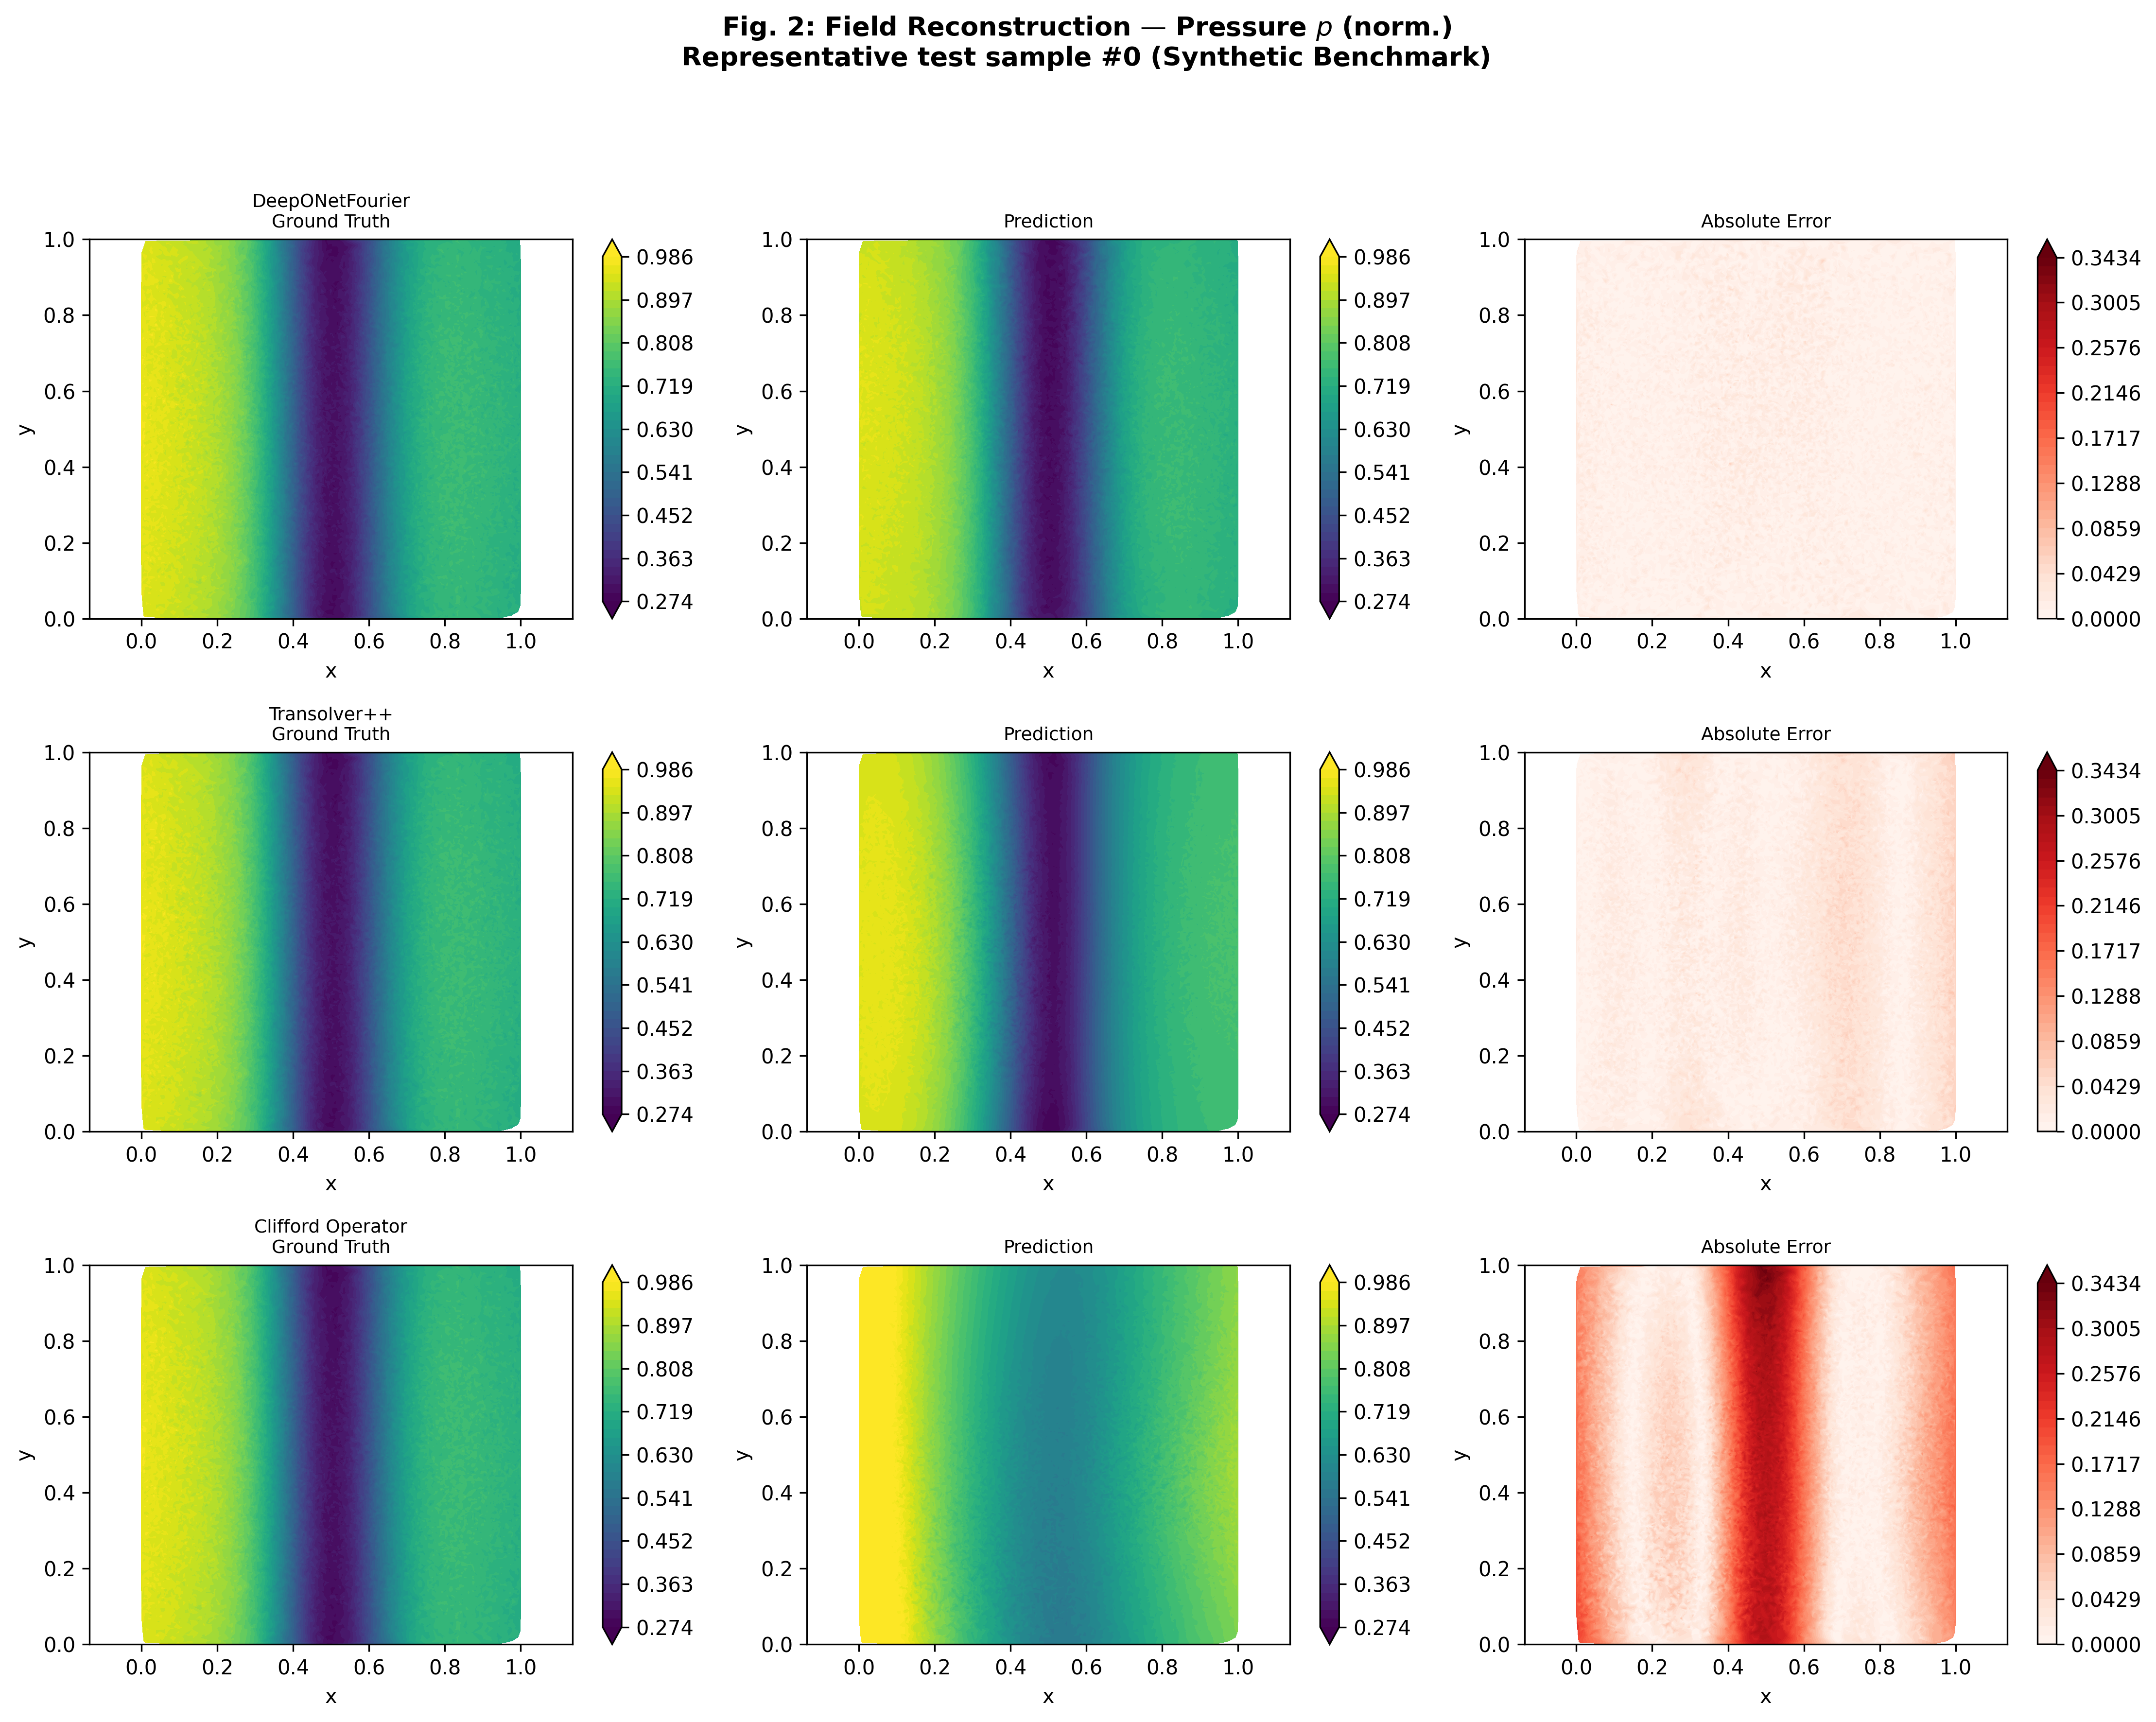
\includegraphics[width=\textwidth]{figures/fig_2_pressure_lossless.png}
\caption{\added{Normalized pressure reconstruction for held-out synthetic case~0. Rows show DeepONetFourier, the Transolver-inspired operator, and the Clifford-algebra operator; columns show common-scale ground truth, common-scale prediction, and common-scale absolute error.}}
\label{fig:pressure_compare}
\end{figure*}

\begin{figure*}[htbp]
\centering
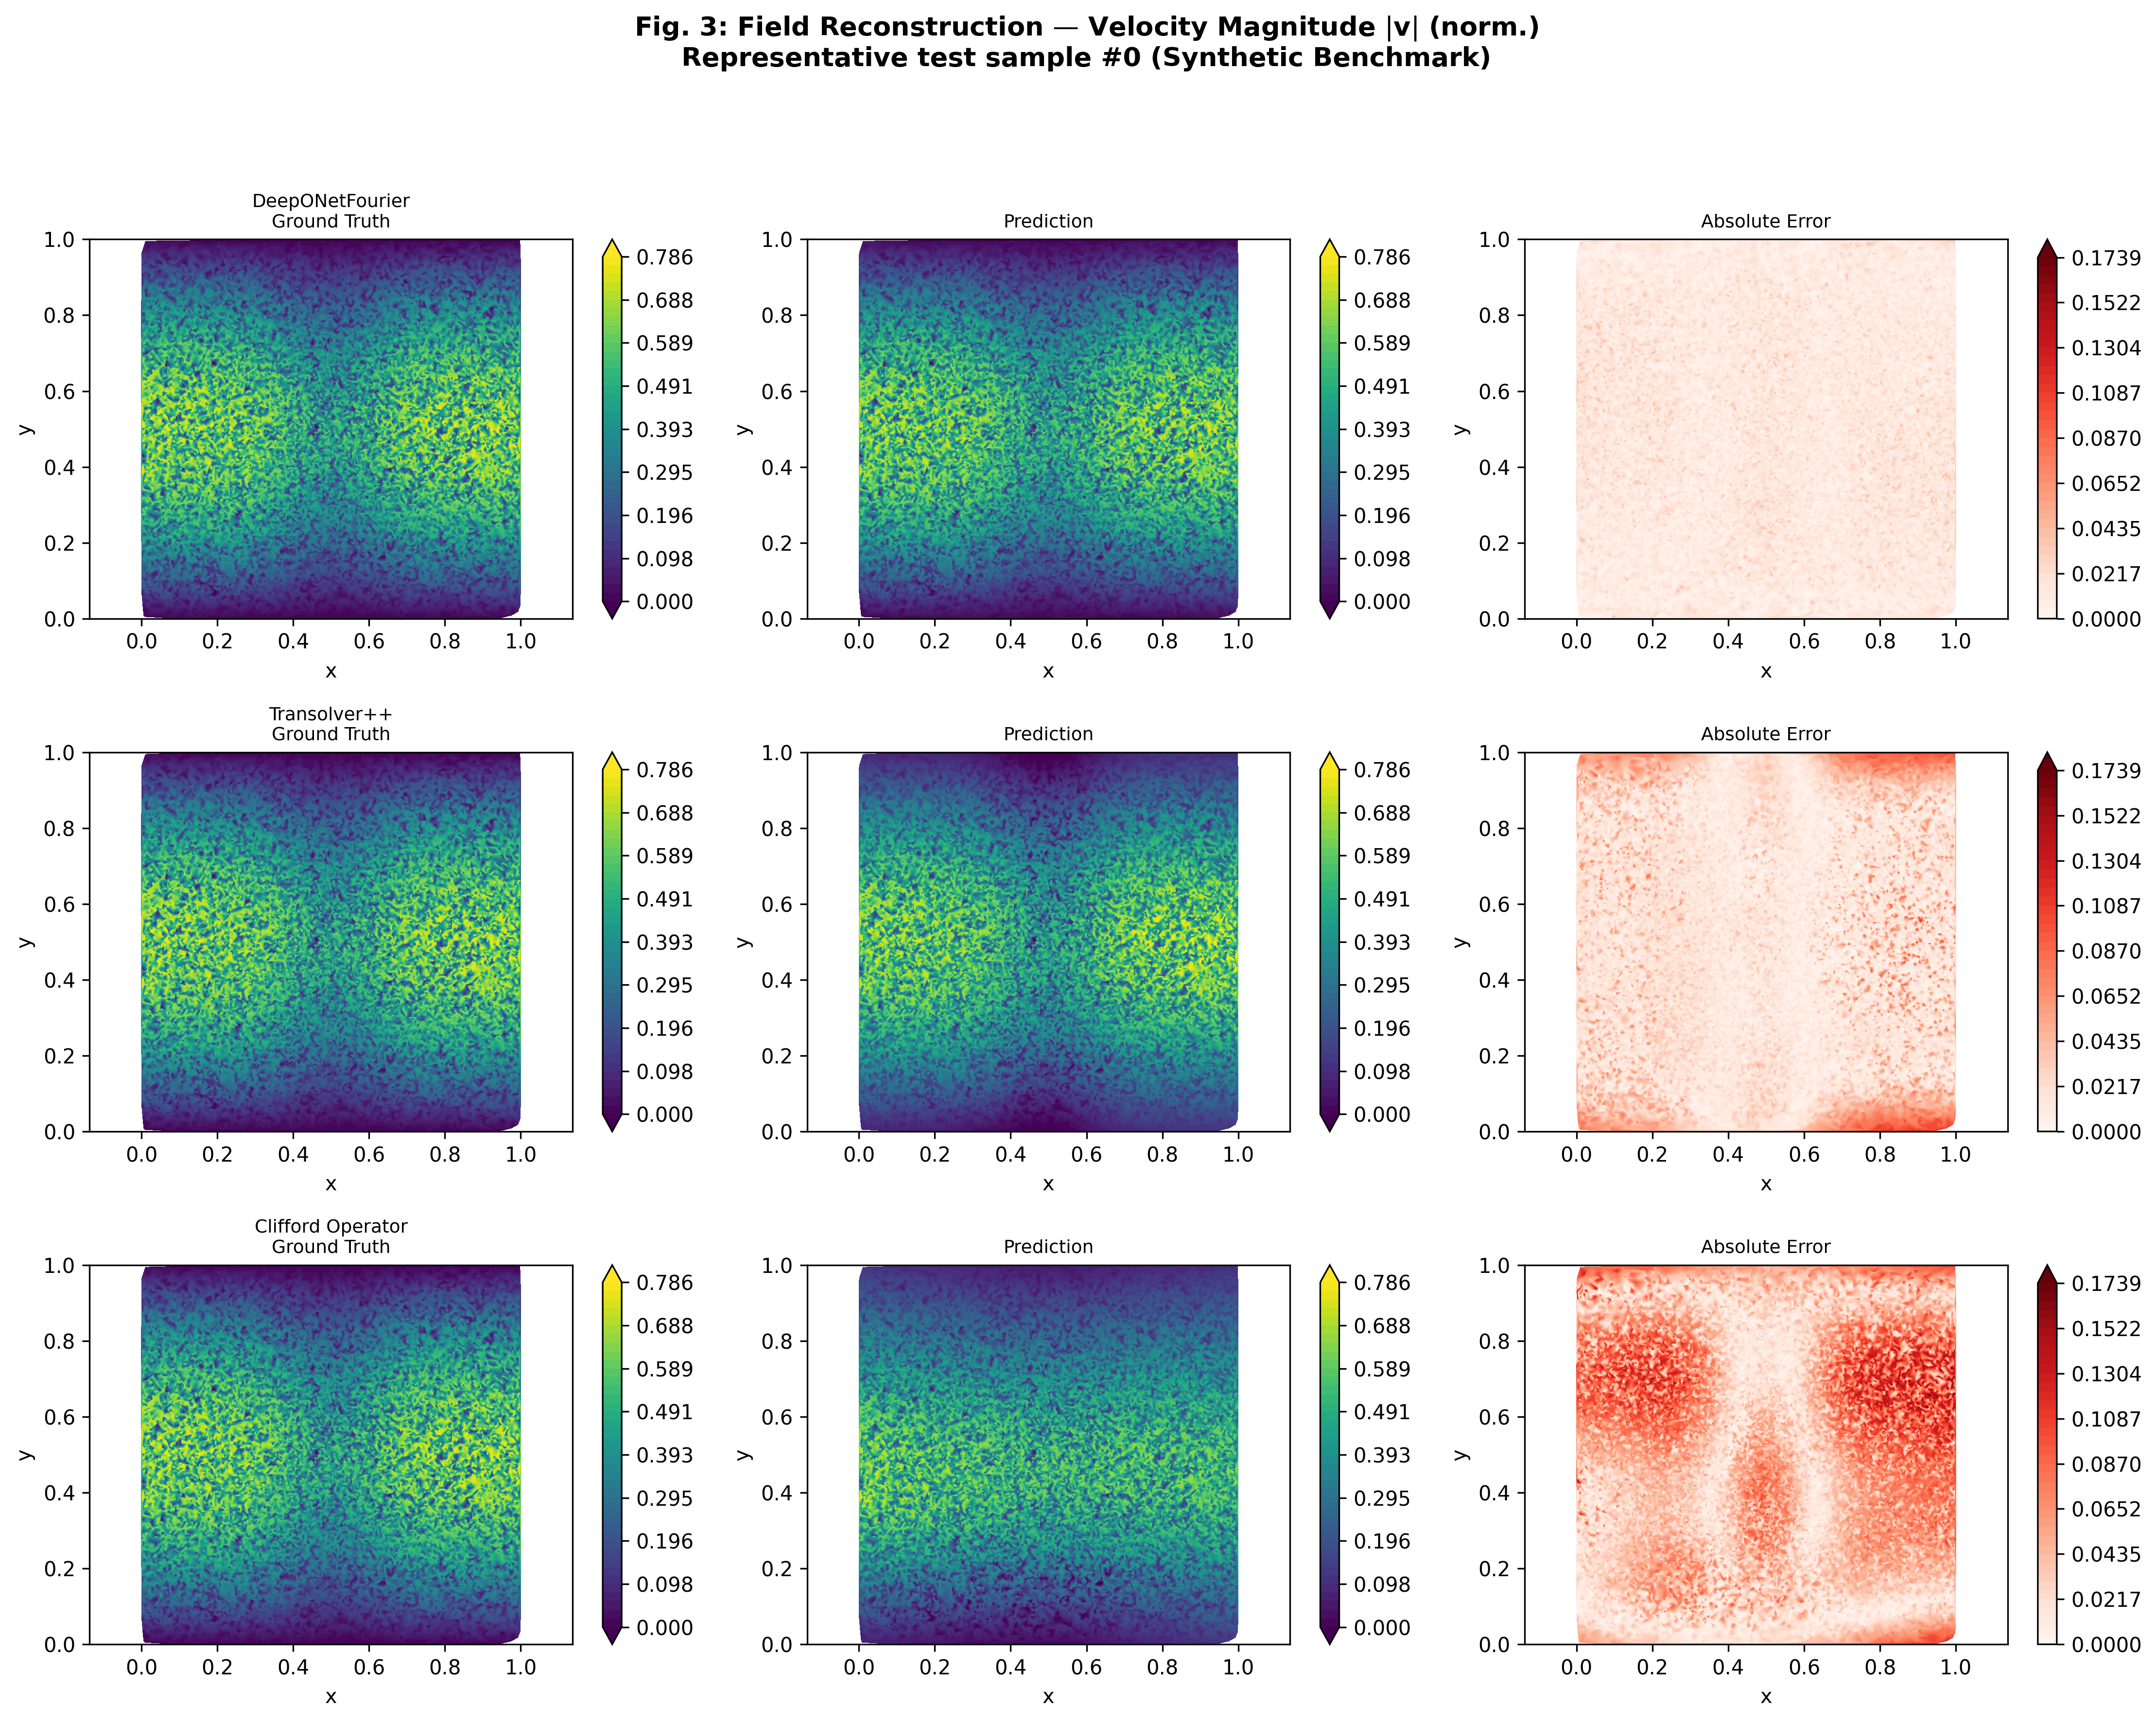
\includegraphics[width=\textwidth]{figures/fig_3_velocity_magnitude_lossless.png}
\caption{\added{Normalized velocity-magnitude reconstruction for held-out synthetic case~0, using the matched layout and scales described in Fig.~\ref{fig:pressure_compare}.}}
\label{fig:velocity_compare}
\end{figure*}

\begin{figure*}[htbp]
\centering
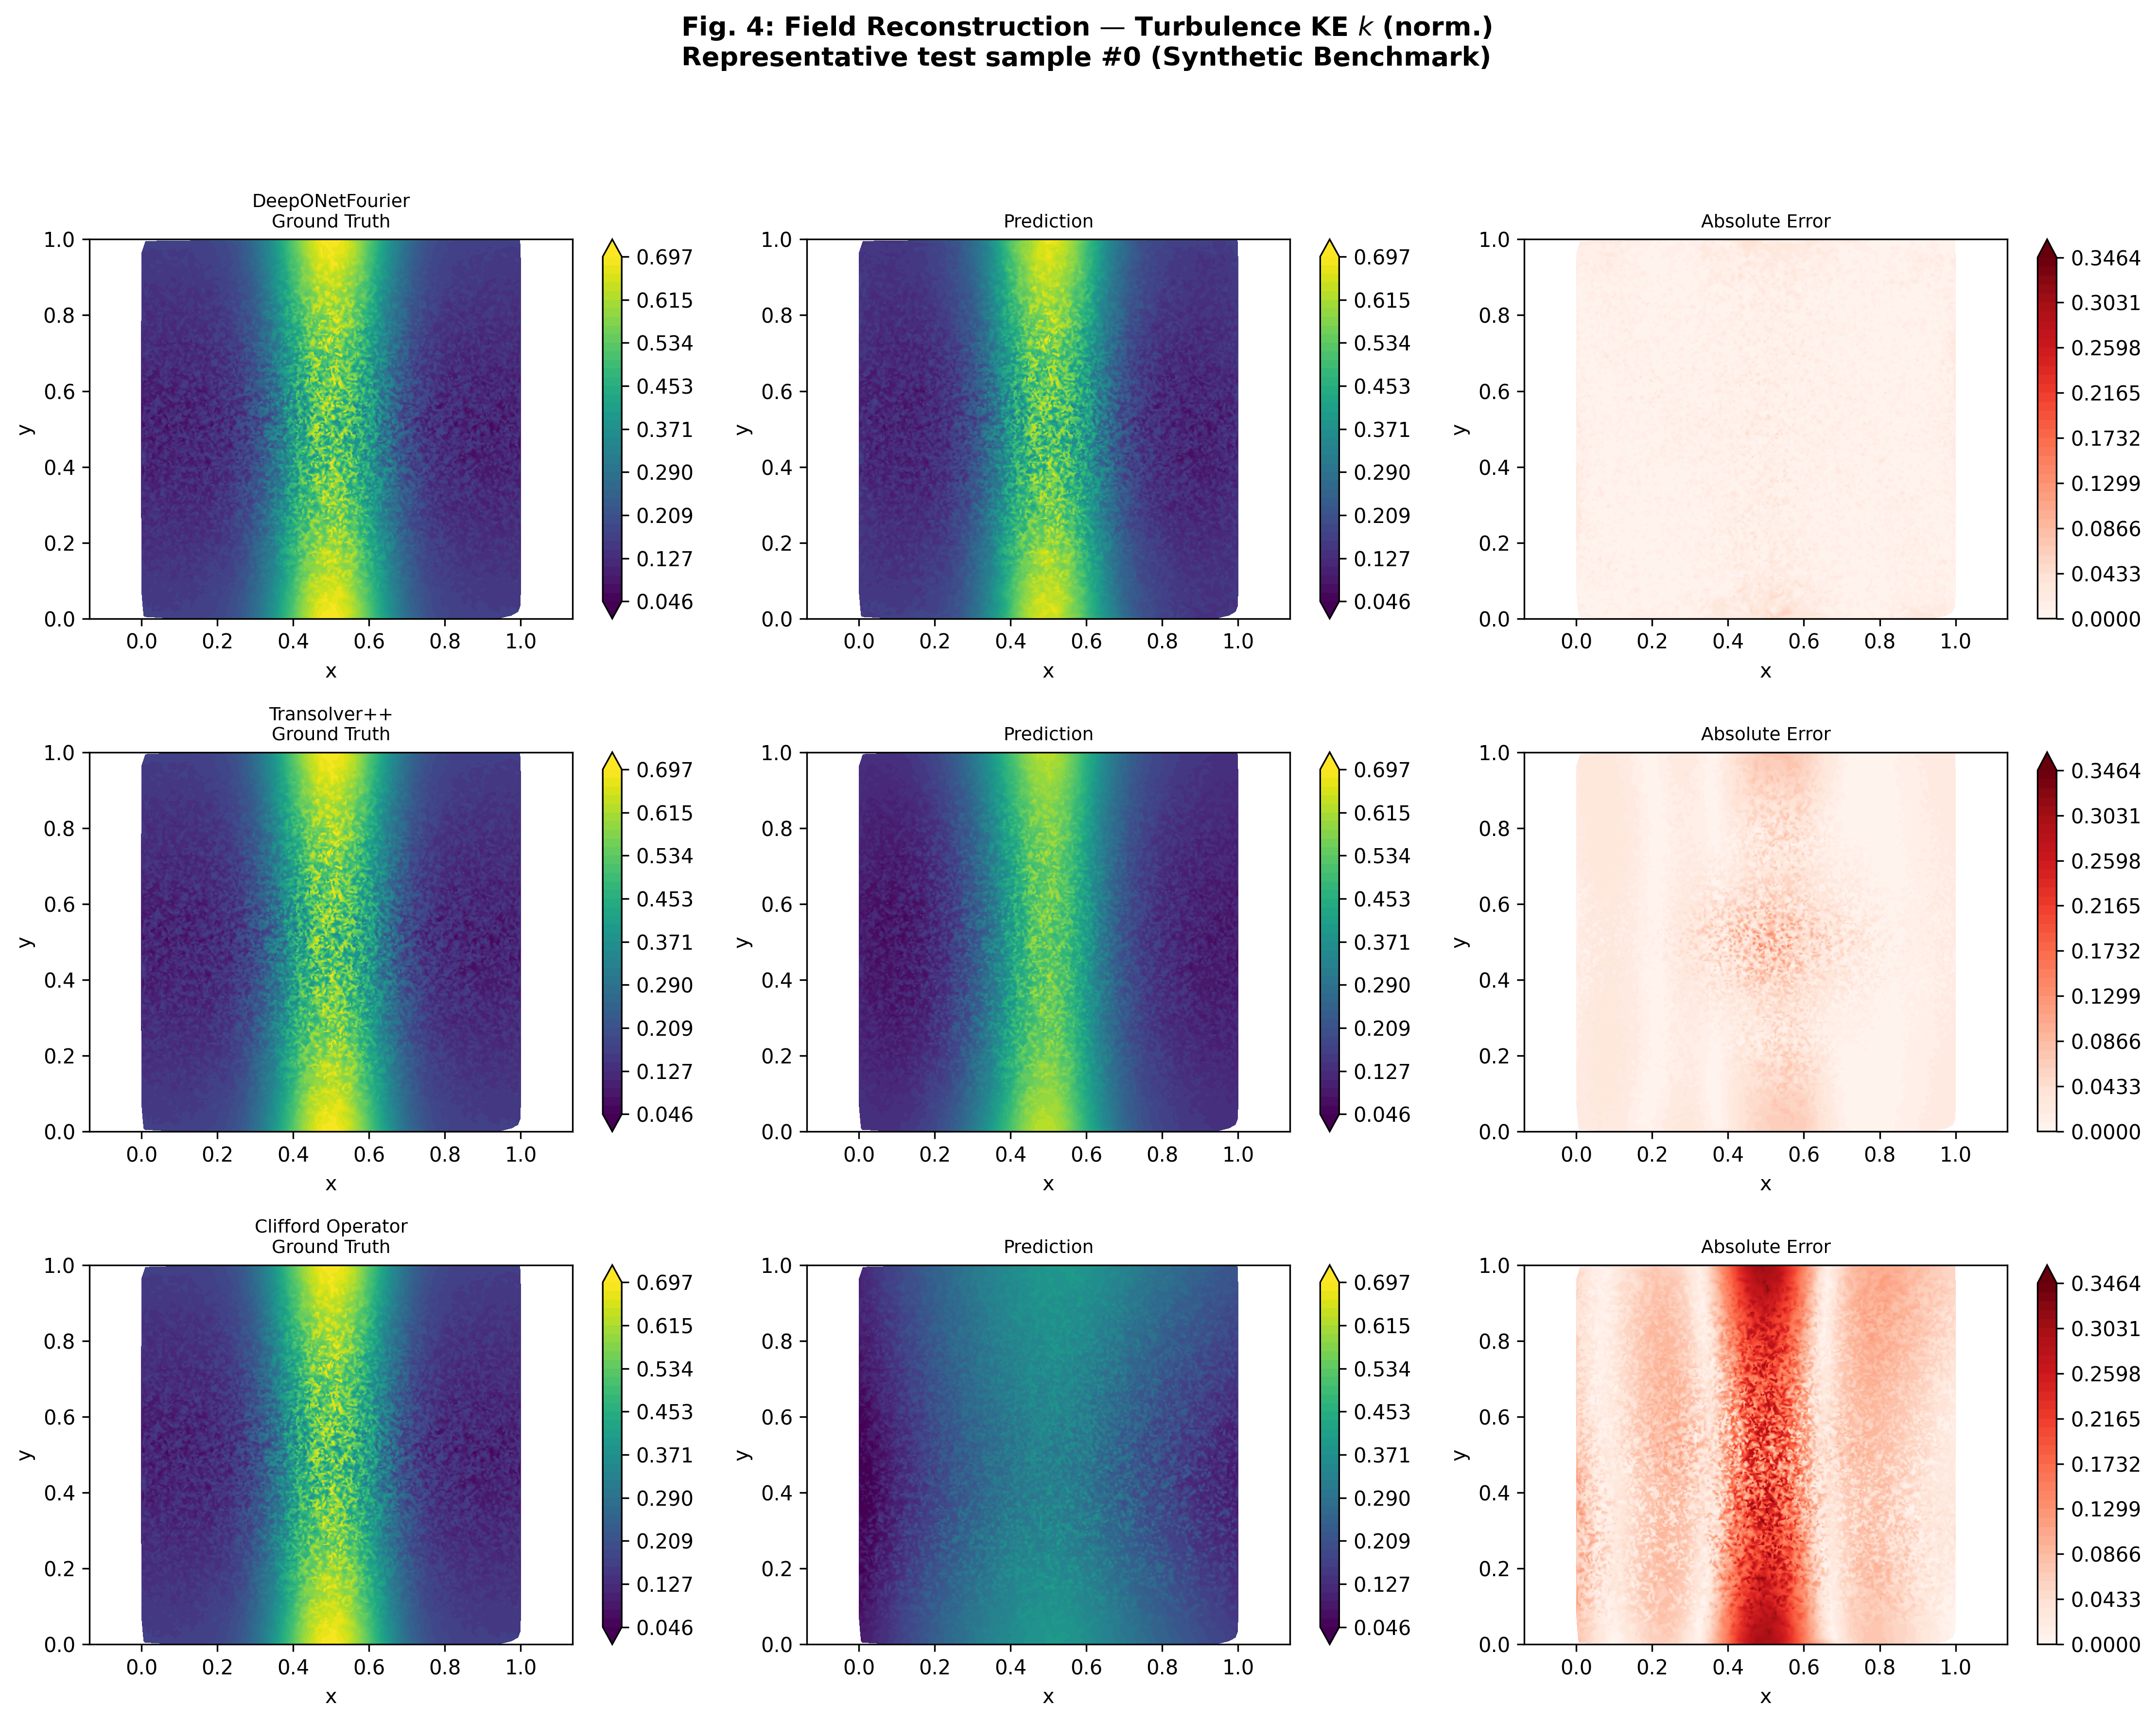
\includegraphics[width=\textwidth]{figures/fig_4_turbulence_k_lossless.png}
\caption{\added{Normalized turbulent-kinetic-energy reconstruction for held-out synthetic case~0, using the matched layout and scales described in Fig.~\ref{fig:pressure_compare}.}}
\label{fig:tke_compare}
\end{figure*}

\begin{figure*}[htbp]
\centering
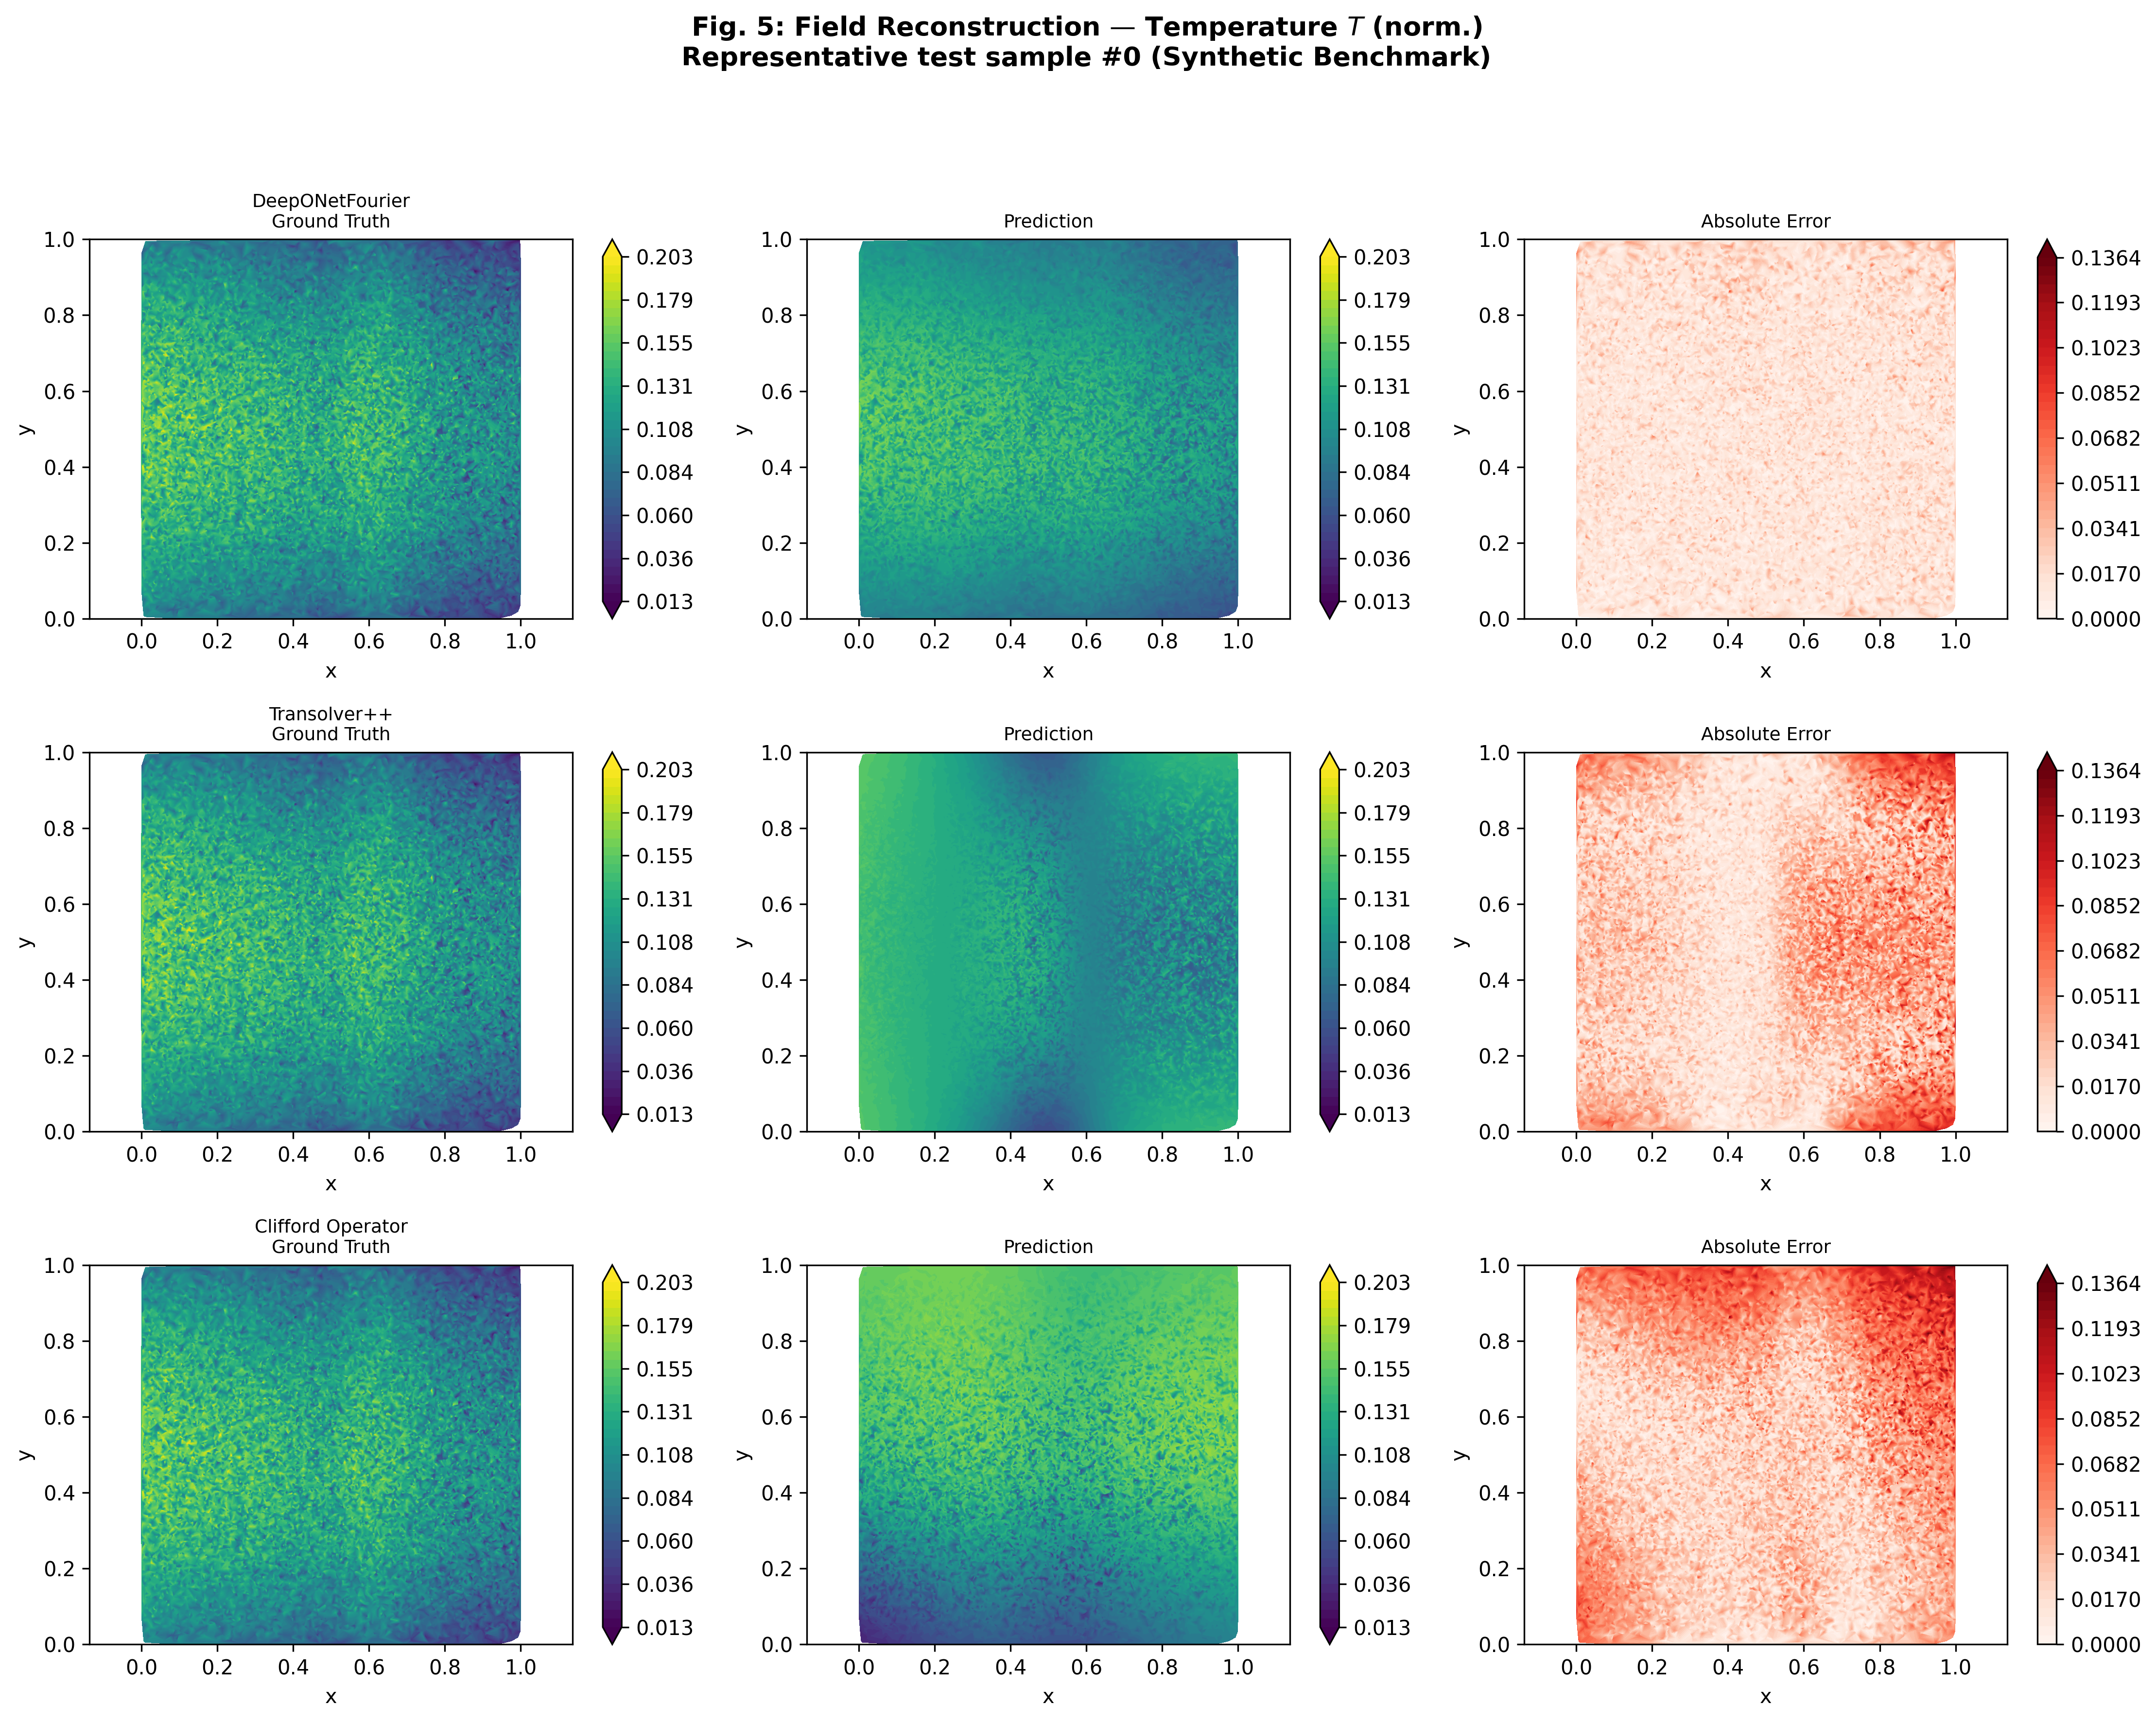
\includegraphics[width=\textwidth]{figures/fig_5_temperature_lossless.png}
\caption{\added{Normalized temperature reconstruction for held-out synthetic case~0, using the matched layout and scales described in Fig.~\ref{fig:pressure_compare}.}}
\label{fig:temperature_compare}
\end{figure*}

Table~\ref{tab:field_metrics} summarizes DeepONetFourier field accuracy on the 300-sample test set under the synthetic benchmark.

\begin{table}[htbp]
\caption{\added{DeepONetFourier pooled field accuracy on all 300 held-out synthetic cases from one archived checkpoint}}
\label{tab:field_metrics}
\centering
\resizebox{\columnwidth}{!}{%
\begin{tabular}{lrrr}
\toprule
\textbf{Field} & \textbf{R$^2$} & \textbf{Rel.\,$L_2$} & \textbf{MAE (norm.)} \\
\midrule
Pressure & \added{0.9961} & \added{0.0158} & \added{0.00947} \\
Velocity magnitude & \added{0.9958} & \added{0.0348} & \added{0.01056} \\
Turbulence $k$ & \added{0.9951} & \added{0.0449} & \added{0.00666} \\
Temperature & \added{0.9962} & \added{0.0278} & \added{0.01221} \\
\bottomrule
\end{tabular}
}
\end{table}

\added{Here, pooled $R^2=1-\sum_i(y_i-\hat y_i)^2/\sum_i(y_i-\bar y)^2$, relative $L_2=\|\hat{\bm y}-\bm y\|_2/\|\bm y\|_2$, and MAE is computed after flattening all cases and nodes for each normalized field. Per-case $R^2$ means (population SD) were 0.9879 (0.0137), 0.9950 (0.0011), 0.9675 (0.0569), and 0.7355 (0.0126), respectively. Temperature's lower per-case $R^2$ reflects its small within-case spatial variance despite high pooled performance; reporting both scopes prevents metric-selection ambiguity.}

\begin{table}[htbp]
\caption{\added{Seed-42 Transolver-inspired pooled field accuracy on all 300 held-out analytic synthetic cases (MSE-only objective)}}
\label{tab:transolver_metrics}
\centering
\resizebox{\columnwidth}{!}{%
\begin{tabular}{lrrr}
\toprule
\added{\textbf{Field}} & \added{\textbf{R$^2$}} & \added{\textbf{Rel.\,$L_2$}} & \added{\textbf{MAE (norm.)}} \\
\midrule
\added{Pressure} & \added{0.991775} & \added{0.022916} & \added{0.013808} \\
\added{Velocity magnitude} & \added{0.993163} & \added{0.044359} & \added{0.012909} \\
\added{Turbulence $k$} & \added{0.980636} & \added{0.089384} & \added{0.012279} \\
\added{Temperature} & \added{0.995113} & \added{0.031441} & \added{0.013671} \\
\bottomrule
\end{tabular}
}
\end{table}

\added{The Transolver-inspired record has a mean across the four pooled field $R^2$ values of 0.990172 and a minimum validation MSE of $3.03474\times10^{-4}$. This fixed-protocol result demonstrates accurate reconstruction across all four fields on the shared analytic benchmark. Architecture-level interpretation remains scoped to the stated objective and test configuration rather than a cross-objective ranking.}

\subsection{Neural Operator Comparison}

\begin{table*}[htbp]
\caption{\added{Neural-operator artifact comparison on the synthetic benchmark with non-identical loss settings}}
\label{tab:benchmark}
\centering
\resizebox{\textwidth}{!}{%
\begin{tabular}{lcccc}
\toprule
\textbf{Metric} & \textbf{DeepONet} & \textbf{DeepONet-F} & \textbf{Transolver} & \textbf{Clifford} \\
\midrule
Total parameters & 3,162,116 & 1,451,012 & \added{3,244,872} & \added{37,380} \\
\added{Retained accuracy evidence} & $R^2$: 0.9933--0.9966 & \added{$R^2$: 0.9951--0.9962} & \added{$R^2$: 0.9806--0.9951} & \added{Case-0 panel} \\
Output shape & $[B,4,N]$ & $[B,4,N]$ & $[B,4,N]$ & $[B,4,N]$ \\
Training objective & MSE & MSE + index proxies & MSE & MSE \\
Evaluated geometry & Fixed mesh & Fixed mesh & Fixed mesh & Fixed mesh \\
\bottomrule
\end{tabular}
}
\end{table*}

\textbf{Key observations under the present benchmark:}
\begin{itemize}
    \item \textbf{DeepONetFourier} reconstructs the four synthetic fields with pooled $R^2=0.9951$--0.9962 on one fixed-mesh checkpoint.  \added{Its different objective prevents attributing any comparative advantage to architecture alone.}
    \item \added{\textbf{The Transolver-inspired operator} supplies global token attention, has 3.245M parameters, and attained pooled $R^2=0.9806$--0.9951 across the four fields in the seed-42 full-test run.}
    \item \added{\textbf{The Clifford-algebra operator} is compact at 37,380 parameters. Those properties require dedicated learning-curve and rotation-consistency experiments.}
\end{itemize}

\subsection{LOCA Indicator Classification Performance}

Fig.~\ref{fig:locac_perf} shows the LOCA indicator classifier performance, and Table~\ref{tab:locac_metrics} summarizes the corresponding metrics. These values evaluate the classifier on PCTRAN-simulated NPPAD rows plus synthetic transition samples; the prescribed break-size parameter is not part of this classifier test. Conversely, when the trained classifier is exercised through the end-to-end translation path, $\eta_\text{eff}$ is dominated by the prescribed break-size term. The classifier result and the translation-path diagnostic therefore establish two complementary components of workflow feasibility, but neither constitutes independent plant-level LOCA validation.

\begin{figure}[htbp]
\centering

\includegraphics[width=\columnwidth]{figures/locac_detection_performance.png}
\caption{\added{Classifier ROC curve (AUC 0.990554), precision--recall curve, and confusion matrix for one seed-42 split of PCTRAN-simulated NPPAD rows plus synthetic transition augmentation. This is classifier-level evidence, not independent end-to-end digital-twin validation.}}
\label{fig:locac_perf}
\end{figure}

\begin{table}[htbp]
\caption{\added{LOCA indicator classifier performance on PCTRAN-simulated NPPAD and synthetic transition data (one seed-42 split)}}
\label{tab:locac_metrics}
\centering
\begin{tabular}{ll}
\toprule
\textbf{Metric} & \textbf{Score} \\
\midrule
Accuracy & \added{0.977374} \\
Precision & \added{0.987281} \\
Recall (Sensitivity) & \added{0.989063} \\
F1 Score & \added{0.988172} \\
ROC-AUC & \added{0.990554} \\
\bottomrule
\end{tabular}
\end{table}

\begin{table}[htbp]
\caption{\added{Five-seed translation-path diagnostic (mean $\pm$ population SD). The direct severity term is removed in the second column, but label-conditioned break size remains an operator input.}}
\label{tab:translation_ablation}
\centering
\begin{tabular}{lcc}
\toprule
\textbf{Metric} & \textbf{80/20 Blend} & \textbf{Direct Term Removed} \\
\midrule
ROC-AUC & 0.999997 $\pm$ 0.000003 & 0.999977 $\pm$ 0.000046 \\
Recall & 1.000000 $\pm$ 0.000000 & 1.000000 $\pm$ 0.000000 \\
F1 & 0.999956 $\pm$ 0.000041 & 0.999989 $\pm$ 0.000022 \\
Accuracy & 0.999912 $\pm$ 0.000082 & 0.999978 $\pm$ 0.000044 \\
\bottomrule
\end{tabular}
\end{table}

 \added{The archived classifier metrics do not retain a break-size-stratified error analysis, and no reliability diagram, Brier score, or expected calibration error was computed. Approximate score-versus-break-size values from the prior draft are therefore omitted rather than presented as calibration evidence. A reliability-oriented follow-up will use independent group-aware splits and report threshold-dependent probability-of-detection/false-alarm curves, proper scoring rules, and calibration intervals.}

\subsection{\added{Runtime Scope}}

\added{The implementation provides explicit timing entry points for both neural-operator execution and the complete single-case path comprising field prediction, feature translation, and classification. A matched timing artifact with warm-up, CUDA synchronization, repeated measurements, software-stack details, and a measured Fluent comparator is not available; consequently, this paper makes no quantitative latency or speedup claim. The existing instrumentation defines a reproducible basis for that benchmark.}

%═══════════════════════════════════════════════════════════════════════════════
\section{Discussion}
\label{sec:discussion}
%═══════════════════════════════════════════════════════════════════════════════

\subsection{Methodological Contributions}

\added{This work makes three primary methodological contributions. First, it demonstrates that three distinct neural-operator paradigms---enhanced branch--trunk decomposition, mesh-token attention, and geometric-algebra encoding---can share one surrogate-to-indicator pipeline. Second, it establishes exact synthetic-test metrics for the archived DeepONetFourier checkpoint, a separately executed seed-42 Transolver-inspired run, and a dataset-matched unmodified DeepONet baseline while documenting the non-identical objectives. Code inspection identifies two index-space proxy terms, preventing a conservation claim and motivating a geometry-aware retraining experiment. Third, it establishes an artifact-traceable evaluation boundary comprising analytic fields, PCTRAN-simulated classifier data, label-conditioned translation, fixed training runs, and explicitly scoped runtime evidence.}

\subsection{Architectural Trade-Off Analysis}

The three architectures address different deployment priorities and the following observations are framed as \emph{preliminary inductive-bias findings} under non-identical optimization settings:

\added{\textbf{DeepONetFourier} has 54.1\% fewer parameters than the retrained DeepONet baseline and achieved pooled $R^2=0.9951$--0.9962 on the 300-case full test set. Fourier encoding is an explicit high-frequency representation mechanism; the incremental effects of that encoding, adaptive activation, and the two proxy terms have not been isolated under matched retraining.}

\added{\textbf{The Transolver-inspired operator} provides global interactions over $M=64$ tokens, with $\mathcal{O}(M^2)$ token-attention complexity, and is the largest studied model at 3.245M parameters. Its fixed seed-42 full-test record attained a mean field $R^2$ of 0.990172, with all four pooled field values above 0.98, supporting the viability of token-mediated global interaction on the shared mesh. Transfer across mesh topology lies outside the present fixed-geometry scope.}

\added{\textbf{The Clifford-algebra operator} is the most compact studied model at 37,380 parameters. Its internal Cl(3,0) operations preserve a useful grade structure, but the dense $256\to4$ decoder mixes grades. Learning-curve and rotation-consistency experiments are required before either advantage can be asserted.}

\subsection{Surrogate-Monitoring Utility and Limits of Current Validation}

\added{The current results measure in-distribution methodological performance under controlled, physics-inspired analytic synthetic conditions. Two boundaries are central to their interpretation:}

\added{The synthetic generator encodes qualitative pipe-flow patterns but does not solve governing equations or establish conservation consistency. The reported DeepONetFourier and Transolver-inspired pooled $R^2$ values therefore quantify interpolation on that analytic generator's distribution, not accuracy relative to Fluent CFD, experiments, or plant transients.}

\added{The blended severity model ($\eta_\text{eff}=0.8\eta_\text{input}+0.2\min(\eta_\text{field},1)$) means the main LOCA score is substantially driven by prescribed break size. The available five-seed ablation removes the explicit translator term, but its break-size input is sampled conditionally on the class. A label-independent evaluation remains necessary to quantify whether reconstructed fields add detection information.}

\subsection{Path to Full-Fidelity Validation}

\added{The repository and present artifacts define a staged route to full-fidelity validation: verify the Fluent automation on the intended elbow geometry; generate an independently quality-controlled case matrix spanning break severity, inlet velocity, and temperature; fit all scalers on training cases only; reserve grouped geometry and operating-condition holdouts; and retrain the operators under matched seeds and objectives. The current Fluent journal-generation and CSV-preprocessing path is an unevaluated prototype, whereas the reported benchmark uses a straight cylindrical analytic proxy. This separation makes the next validation stage explicit and reproducible.}

\subsection{Limitations and Future Work}
\label{sec:limitations}

\textbf{Missing baselines}:  \added{A dataset-matched unmodified DeepONet result is now included, but plain MLP and FNO baselines remain absent. A component ablation is also required to isolate Fourier features, adaptive activations, and each proxy term.}

\added{\textbf{Statistical scope}: The study prioritizes end-to-end method integration and artifact-level reproducibility; field metrics therefore characterize fixed archived runs, while the constrained translation-path diagnostic uses five seeds. The reported values support feasibility on the prescribed split but are not confidence intervals or tests of statistically significant differences between architectures. Repeated training under matched objectives and compute budgets is reserved for a larger comparative study.}

\textbf{Split and preprocessing protocol}: \added{The current field split samples randomly from a regular parameter grid and therefore tests in-distribution interpolation rather than extrapolation to a held-out operating regime. In addition, the current preprocessor fits min--max scalers before partitioning, so held-out extrema influence scaling. The classifier uses a row-level split that can place time steps from one simulated transient in both training and test sets. Future validation will fit preprocessing on training data only and use parameter-blocked field splits and transient-grouped classifier splits.}

\textbf{Non-identical optimization}: DeepONetFourier uses a doubled value-fidelity term plus index-gradient and velocity-variation proxies, whereas the other operators use MSE only. A controlled comparison requires matched objectives and tuning budgets; present cross-architecture figures are qualitative artifact inspections, not a ranking.

\textbf{Steady-state assumption}: LOCA events are transient, and the present results address only steady-state field reconstruction.  \added{No enabled configuration, checkpoint, or transient result was found for the prototype temporal module; temporal operator learning is therefore future work. Evaluation should use transient CFD and independently aligned sensor sequences and report detection delay, probability of detection, false alarms, and distribution-shift performance.}

\textbf{Uncertainty quantification}: The evaluated pipeline produces point predictions and classifier scores only.  \added{Diffusion is disabled by default; no trained diffusion checkpoint, held-out sampling protocol, coverage result, or decision-level propagation artifact was found. DDPM-based turbulence sampling is therefore future work, and a classifier score is not predictive uncertainty. A complete study must report nominal versus empirical coverage, interval width, proper scores, and calibration and propagate uncertainty through feature translation and classification.}

\textbf{Detection-threshold and false-alarm analysis}: The classifier currently reports performance at a single decision threshold (0.5) via aggregate metrics (ROC-AUC, recall, F1). A reliability-oriented treatment should additionally report the detection-threshold/false-alarm-rate trade-off explicitly (e.g., an operating-point analysis tied to an acceptable false-alarm budget for operator-facing screening), since false negatives and false positives carry very different consequences in a LOCA-screening context.

\textbf{AI-model failure modes}: This study does not analyze distribution shift between analytic synthetic fields and Fluent/experimental data, robustness to noise or simulator shift in the PCTRAN-derived features, or behavior outside $v\in[4.0,6.0]$\,m/s, $b\in[0,10]\%$, and $T\in[290,320]^\circ$C. Such evidence is central to a reliability argument \cite{nrc7294,trilateral2024}.

\textbf{Multi-fidelity learning}: A residual multi-fidelity module combining coarse-RANS and fine-LES predictions ($u_\text{final} = u_\text{base} + u_\text{residual}$) is a planned extension; not evaluated in the present results.

\textbf{Wall shear stress}: A post-processing module for $\tau_w = \mu\,\partial u/\partial y$ with corrosion-risk assessment is a planned extension for pipe-integrity monitoring; not evaluated in the present results.

%═══════════════════════════════════════════════════════════════════════════════
\section{Conclusion}
\label{sec:conclusion}
%═══════════════════════════════════════════════════════════════════════════════

\added{This paper has presented a proof-of-concept, multi-architecture neural-operator workflow for Cold-Leg LOCA screening in the AP1000 PWR, comparing three operator paradigms and coupling the archived DeepONetFourier surrogate to a downstream classification pipeline. The principal findings were obtained under the physics-inspired analytic synthetic benchmark described in Section~\ref{sec:problem}:}

\begin{itemize}
    \item \added{\textbf{DeepONetFourier} has 1,451,012 parameters, 54.1\% fewer than the 3,162,116-parameter retrained DeepONet baseline. Its archived checkpoint attains pooled test $R^2=0.9951$--0.9962 across the four analytic synthetic fields. Fourier coordinates and adaptive activations are combined with two explicitly scoped index-space regularizers.}
    \item \added{\textbf{The Transolver-inspired operator} has 3,244,872 parameters and provides global attention over 64 learned mesh tokens. Its separately archived seed-42 MSE-only run attained pooled test $R^2=0.9806$--0.9951 across the four analytic synthetic fields (mean 0.990172), supporting token-based global interaction as a viable fixed-mesh surrogate mechanism.}
    \item \added{\textbf{The Clifford-algebra operator} is the most compact studied architecture at 37,380 parameters, approximately $38.8\times$ fewer than DeepONetFourier. Its internal multivector operations provide a grade-structured inductive bias; rotation-aware decoding remains to be evaluated.}
    \item The single-split classifier artifact reaches ROC-AUC 0.990554, recall 0.989063, and F1 0.988172 on PCTRAN-simulated NPPAD rows plus synthetic transition augmentation. The five-seed translation-path ablation remains label-conditioned, so neither result establishes independent LOCA detection from predicted fields.
    \item \added{The implementation provides a unified single-case inference and timing path for all three architectures. Quantitative speedup is reserved for a matched benchmark with archived timing distributions and a measured CFD reference.}
\end{itemize}

\added{Collectively, these results establish a reproducible, artifact-traceable proof of concept for multi-architecture field reconstruction and surrogate-to-indicator integration. The shared configuration interface, exact held-out metrics, and explicit evidence boundaries provide a concrete foundation for full-fidelity CFD or experimental validation, geometry-aware physical derivatives, label-independent detection, independent replication, calibrated uncertainty, and a reliability safety case.}

%─── Data Availability ────────────────────────────────────────────────────────
\section*{Data Availability Statement}
\added{Project source code, including the analytic synthetic-field generator, is publicly available at \url{https://github.com/Punyansh26/Digital-Twin-for-NPP-Cold-Leg-LOCAC-detection}. The exact local split, checkpoints, metric JSON files, and revised figures used for this manuscript are available from the corresponding author upon reasonable request. The PCTRAN-simulated NPPAD collection is openly available under the Creative Commons Attribution 4.0 license from the originating publication and Figshare record \cite{qi2022nppad}; DOI: \url{https://doi.org/10.6084/m9.figshare.c.6238473}.}

%─── Acknowledgment ───────────────────────────────────────────────────────────
\section*{Acknowledgment}
\added{The authors acknowledge Qi \emph{et al.}~\cite{qi2022nppad} for the open PCTRAN-simulated NPPAD time-series dataset used in the classifier study. The physics-inspired analytic synthetic field generator used for neural-operator training and evaluation was developed as part of this project. Computational resources for the archived training runs included an NVIDIA RTX~4060 GPU.}

%─── References ───────────────────────────────────────────────────────────────
\begin{thebibliography}{00}

\bibitem{lu2021deeponet}
L. Lu, P. Jin, G. Pang, Z. Zhang, and G. E. Karniadakis,
``Learning nonlinear operators via DeepONet based on the universal approximation theorem of operators,''
\textit{Nature Machine Intelligence}, vol.~3, pp.~218--229, 2021.

\bibitem{chen1995}
T. Chen and H. Chen,
``Universal approximation to nonlinear operators by neural networks with arbitrary activation functions and its application to dynamical systems,''
\textit{IEEE Trans.\ Neural Networks}, vol.~6, no.~4, pp.~911--917, 1995.

\bibitem{lu2022comprehensive}
\added{L. Lu, X. Meng, S. Cai, Z. Mao, S. Goswami, Z. Zhang, and G. E. Karniadakis,
``A comprehensive and fair comparison of two neural operators (with practical extensions),''
\textit{Comput.\ Methods Appl.\ Mech.\ Engrg.}, vol.~393, p.~114778, 2022.}

\bibitem{li2021fno}
Z. Li, N. Kovachki, K. Azizzadenesheli, B. Liu, K. Bhattacharya, A. Stuart, and A. Anandkumar,
``Fourier neural operator for parametric partial differential equations,''
in \textit{Proc.\ ICLR}, 2021.

\bibitem{wu2024transolver}
H. Wu, H. Luo, H. Wang, J. Wang, and M.~Long,
``Transolver: A fast transformer solver for PDEs on general geometries,''
in \textit{Proc.\ ICML}, 2024.

\bibitem{brandstetter2023clifford}
\added{J. Brandstetter, R. van den Berg, M. Welling, and J. K. Gupta,
``Clifford neural layers for PDE modeling,''
in \textit{Proc.\ ICLR}, 2023.}

\bibitem{rahaman2019spectral}
N. Rahaman, A.~Baratin, D.~Arpit, F.~Draxler, M.~Lin, F.~Hamprecht, Y.~Bengio, and A.~Courville,
``On the spectral bias of neural networks,''
in \textit{Proc.\ ICML}, pp.~5301--5310, 2019.

\bibitem{tancik2020ffn}
M. Tancik et~al.,
``Fourier features let networks learn high frequency functions in low dimensional domains,''
in \textit{Proc.\ NeurIPS}, 2020.

\bibitem{son2021sobolev}
H. Son, J. W. Jang, W. J. Han, and H. J. Hwang,
``Sobolev training for physics-informed neural networks,''
\textit{arXiv:2101.08932}, 2021.

\bibitem{wecdcd}
Westinghouse Electric Company,
``AP1000 Design Control Document (DCD),''
NRC ADAMS ML11171A500, Rev.~19, 2011.

\bibitem{nrc_loca}
\added{U.S. Nuclear Regulatory Commission,
``Best-estimate calculations of emergency core cooling system performance,''
Regulatory Guide 1.157, May 1989.}

\bibitem{grieves2014}
M. Grieves and J. Vickers,
``Digital twin: Mitigating unpredictable, undesirable emergent behavior in complex systems,''
in \textit{Transdiscipl.\ Perspectives Complex Syst.}, Springer, 2017, pp.~85--113.

\bibitem{huang2023review}
\added{Q. Huang, S. Peng, J. Deng, H. Zeng, Z. Zhang, Y. Liu, and P. Yuan,
``A review of the application of artificial intelligence to nuclear reactors: Where we are and what's next,''
\textit{Heliyon}, vol.~9, no.~3, Art.~no.~e13883, 2023, doi: 10.1016/j.heliyon.2023.e13883.}

\bibitem{hao2023gnot}
Z. Hao et~al.,
``GNOT: A general neural operator transformer for operator learning,''
in \textit{Proc.\ ICML}, 2023.

\bibitem{hossain2025virtual}
\added{R. Hossain, F. Ahmed, K. Kobayashi, S. Koric, D. Abueidda, and S. B. Alam,
``Virtual sensing-enabled digital twin framework for real-time monitoring of nuclear systems leveraging deep neural operators,''
\textit{npj Materials Degradation}, vol.~9, Art.~no.~21, 2025, doi: 10.1038/s41529-025-00557-y.}

\bibitem{lee2026hcsg}
\added{M. Lee, S. Oh, C. Song, B. Cho, S. Baral, S. Khanal, M. Song, and J. Jeon,
``Neural operator-based surrogate model for CFD: Helical coil steam generator in small modular reactor,''
\textit{arXiv:2605.30277}, 2026, doi: 10.48550/arXiv.2605.30277.}

\bibitem{qi2022nppad}
\added{B. Qi, X. Xiao, J. Liang, L.-C. Po, L. Zhang, and J. Tong,
``An open time-series simulated dataset covering various accidents for nuclear power plants,''
\textit{Scientific Data}, vol.~9, Art.~no.~766, 2022, doi: 10.1038/s41597-022-01879-1.}

\bibitem{isermann2005}
\added{R. Isermann,
``Model-based fault-detection and diagnosis---status and applications,''
\textit{Annual Reviews in Control}, vol.~29, no.~1, pp.~71--85, 2005, doi: 10.1016/j.arcontrol.2004.12.002.}

\bibitem{ieee1012}
\added{\textit{IEEE Standard for System, Software, and Hardware Verification and Validation},
IEEE Std 1012-2016, 2017.}

\bibitem{nrc7294}
\added{Z. Ma, H. Bao, S. Zhang, M. Xian, and A. Mack,
``Exploring advanced computational tools and techniques with artificial intelligence and machine learning in operating nuclear plants,''
NUREG/CR-7294, INL/EXT-21-61117, U.S. Nuclear Regulatory Commission, Feb.~2022. [Online]. Available: \url{https://www.nrc.gov/reading-rm/doc-collections/nuregs/contract/cr7294/index}}

\bibitem{trilateral2024}
 \added{Canadian Nuclear Safety Commission, U.K. Office for Nuclear Regulation, and U.S. Nuclear Regulatory Commission,
``Considerations for developing artificial intelligence systems in nuclear applications,'' Aug.~2024. [Online]. Available: \url{https://onr.org.uk/media/03zl1osf/canukus_trilateral_ai_principles_paper_2024_08_28-final.pdf}
}

\bibitem{petruzzi2008}
\added{A. Petruzzi and F. D'Auria,
``Thermal-hydraulic system codes in nuclear reactor safety and qualification procedures,''
\textit{Science and Technology of Nuclear Installations}, vol.~2008, Art.~no.~460795, 2008, doi: 10.1155/2008/460795.}

\bibitem{nrc_codes}
\added{U.S. Nuclear Regulatory Commission,
``Computer codes,'' [Online]. Available: \url{https://www.nrc.gov/about-nrc/regulatory/research/safety-codes.html}. Accessed: Aug.~31, 2026.
}

\end{thebibliography}

%─── Author Biographies ────────────────────────────────────────────────────────
\begin{IEEEbiographynophoto}{Punyansh Thakur}
is a third-year undergraduate student in the Data Science and Artificial Intelligence program at IIIT Naya Raipur, India. His academic work in this project focuses on neural-operator surrogate modeling, scientific machine learning, and digital-twin workflows for engineering systems.
\end{IEEEbiographynophoto}

\begin{IEEEbiographynophoto}{Anushka Paul}
is a third-year undergraduate student in the Data Science and Artificial Intelligence program at IIIT Naya Raipur, India. Her academic work in this project focuses on data-driven thermohydraulic analysis and machine-learning methods for reliability-oriented accident screening.
\end{IEEEbiographynophoto}

\begin{IEEEbiographynophoto}{Ayush Kumar Bhadra}
is a third-year undergraduate student in the Electronics and Communication Engineering program at IIIT Naya Raipur, India. His academic work in this project focuses on integrating engineering-domain knowledge with data-driven field reconstruction and system-indicator analysis.
\end{IEEEbiographynophoto}

\begin{IEEEbiographynophoto}{Vinay Kumar}
is an Assistant Professor in the Department of Computer Science and Engineering at IIIT Naya Raipur, India. He received his doctoral degree in computer science and engineering from the Indian Institute of Technology (BHU), Varanasi, India. Before joining IIIT Naya Raipur, he served as an Assistant Professor at the National Institute of Technology Jamshedpur and Birla Institute of Technology Mesra, Ranchi. He has authored or coauthored more than 30 papers in peer-reviewed journals and conference proceedings and has served as a reviewer for international journals and conferences. His research interests include reliability, safety, and mathematical modeling.
\end{IEEEbiographynophoto}

\end{document}
